\section{Results} \label{sec:result}
\subsection{Subsampling Strategy}
We first evaluate the convergence and effectiveness of the proposed subsampling strategy, and compare it with the state-of-the-art frequency solver~\cite{heide2015fast}. The proposed algorithm, with different sub-sampling factors, was tested on the fruit dataset~\cite{zeiler2010deconvolutional} which contains 10 training images in the size of $100 \times 100$. The dictionary dimension size is set to $11 \times 11 \times 100$.

{\bfseries Convergence.} Comparisons of the convergence between the proposed method and the state-of-the-art are shown in Fig.~\ref{fig:subsampleResult}. A different selection of the subsampling probability reveals that the proposed strategy will slightly influence the convergence and the training objective of the minimization problem. Specifically, the more subsampled, the relatively slower convergence and the higher objective will be obtained. On the other hand, small subsampling rate will significantly accelerate the computation process, where $10\%$ subsampling achieves about $6 \times$ speedup over no subsampled solver and $2 \times$ speedup over state-of-the-art frequency solver for one iteration. We observe that a subsampling rate between $0.1$ and $0.2$ delivers empirically good enough convergence in our settings, as well as achieving at least $3 \times$ speedup. In general, the proposed method converges within 10 iterations, while the comparable method requires roughly 13 iterations to reach converge. Notice that the comparable method has a relatively high objective at first $6-8$ iterations due to different splitting strategies are applied and subproblems are interleaved on the primary variables~\cite{wohlberg2016efficient}, though it converges to an optimum with comparable objective after 10 iterations. In summary, comparing to the state-of-the-art frequency solver, the proposed method with a subsampling rate of $10\%$ not only spends two times less processing time per iteration, but also needs fewer iterations to converge.

\begin{figure}[h]
\begin{subfigure}{0.6\textwidth}
  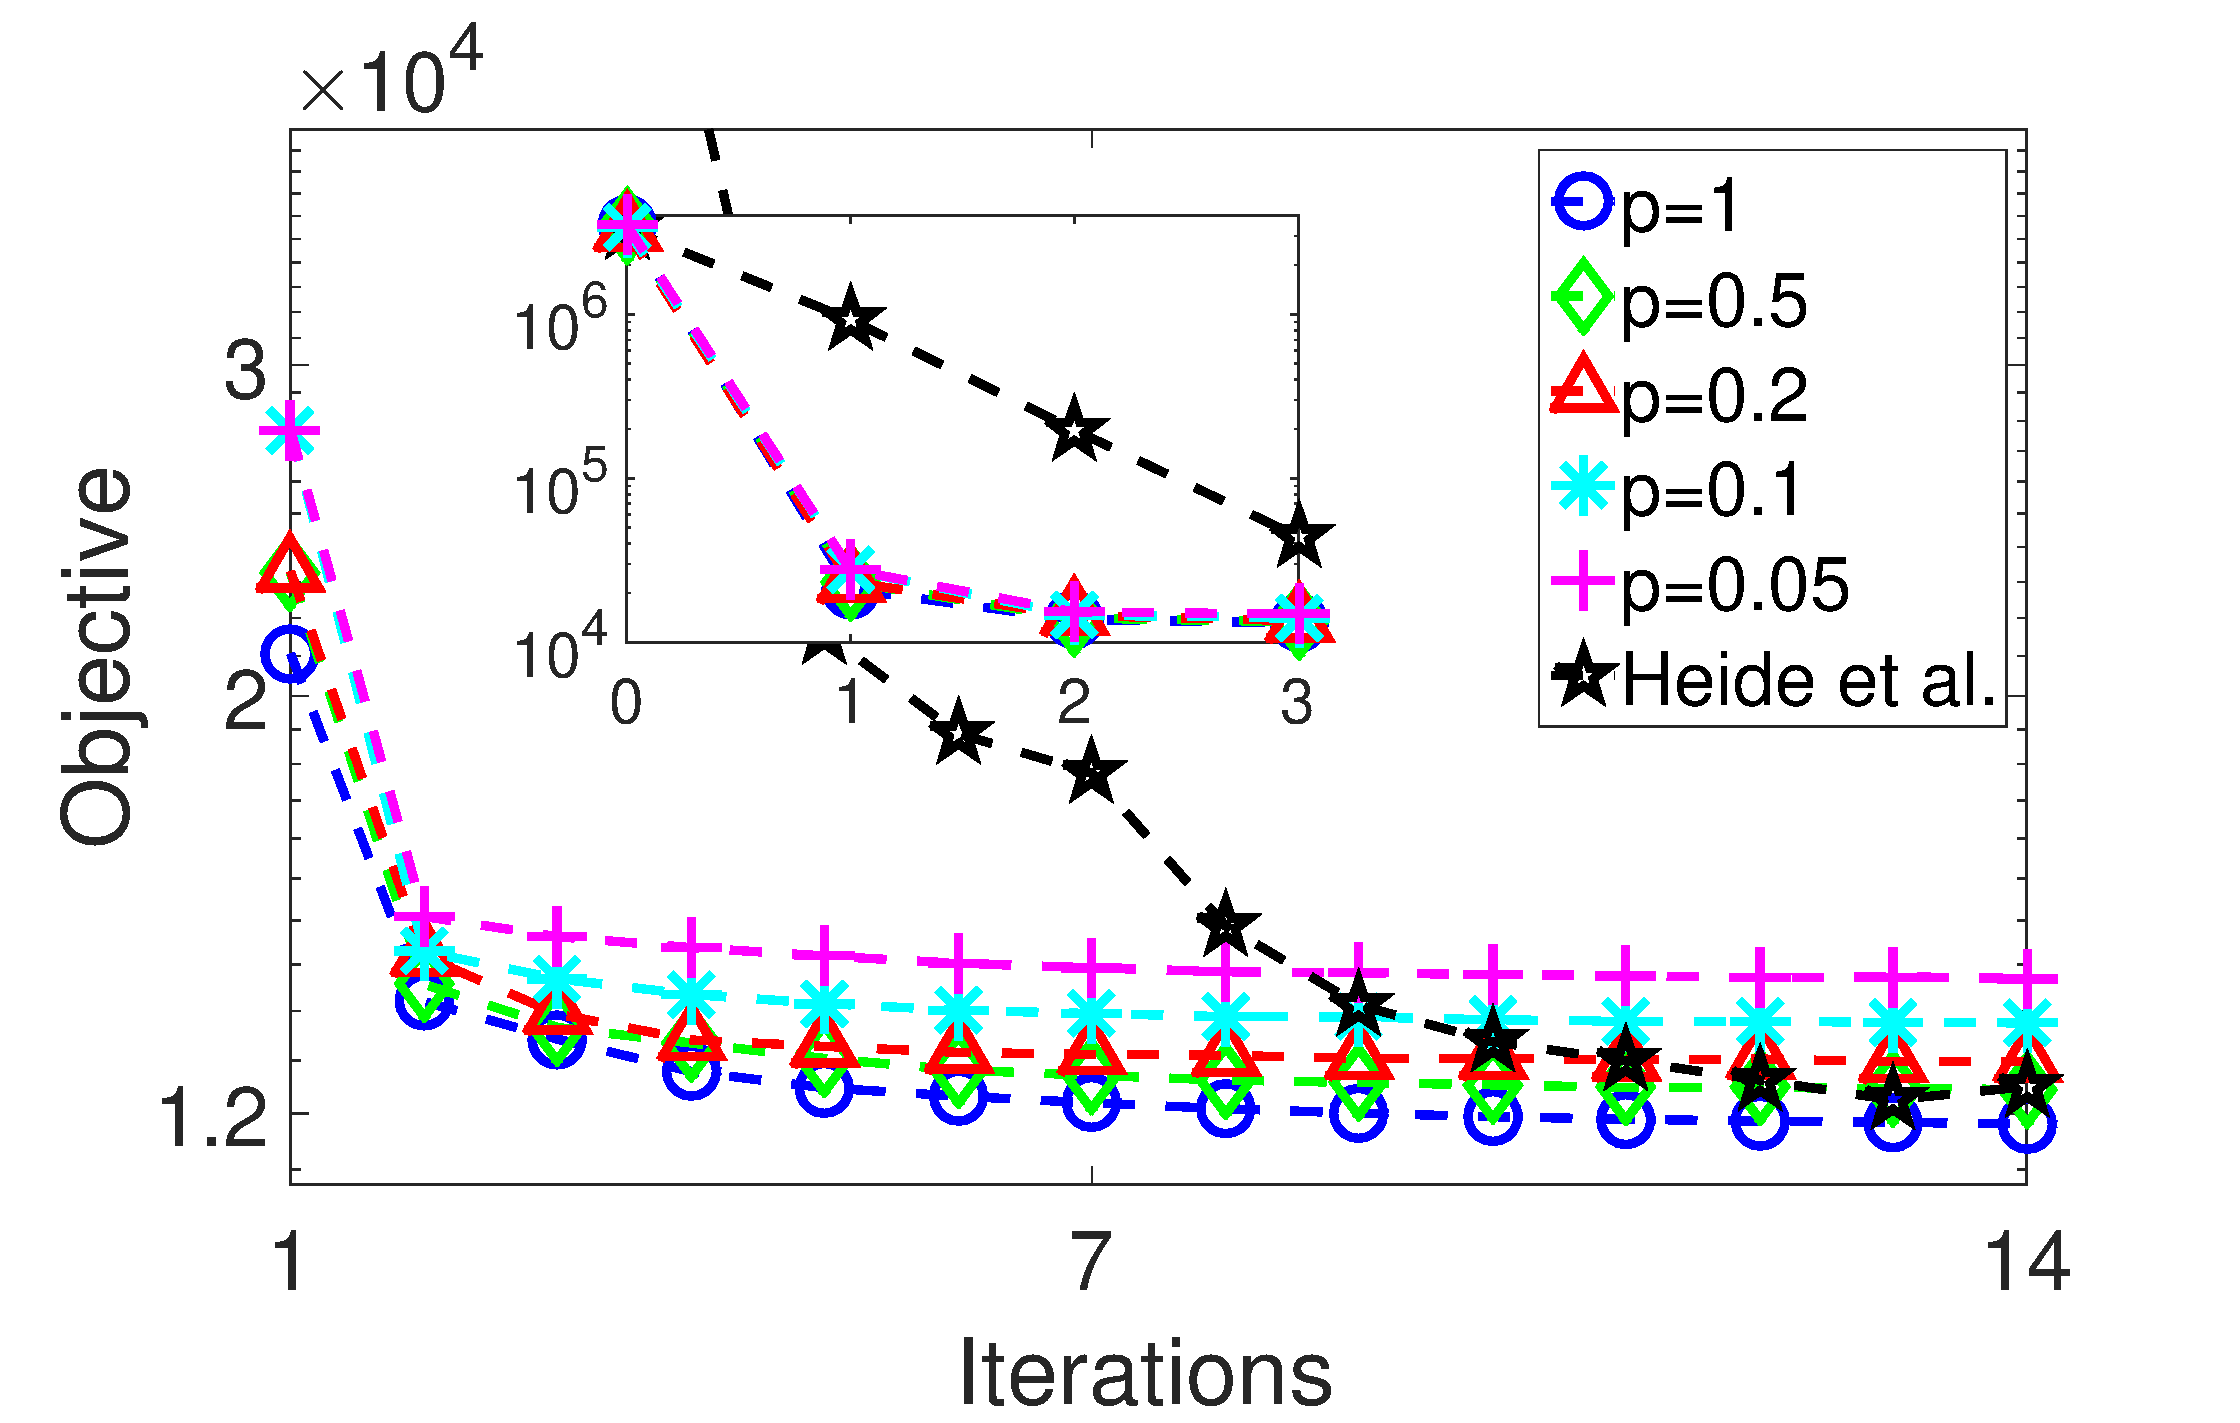
\includegraphics[width=1\linewidth]{figure/iteVSobj.pdf}
\end{subfigure} 
\begin{subfigure}{0.3\textwidth}
  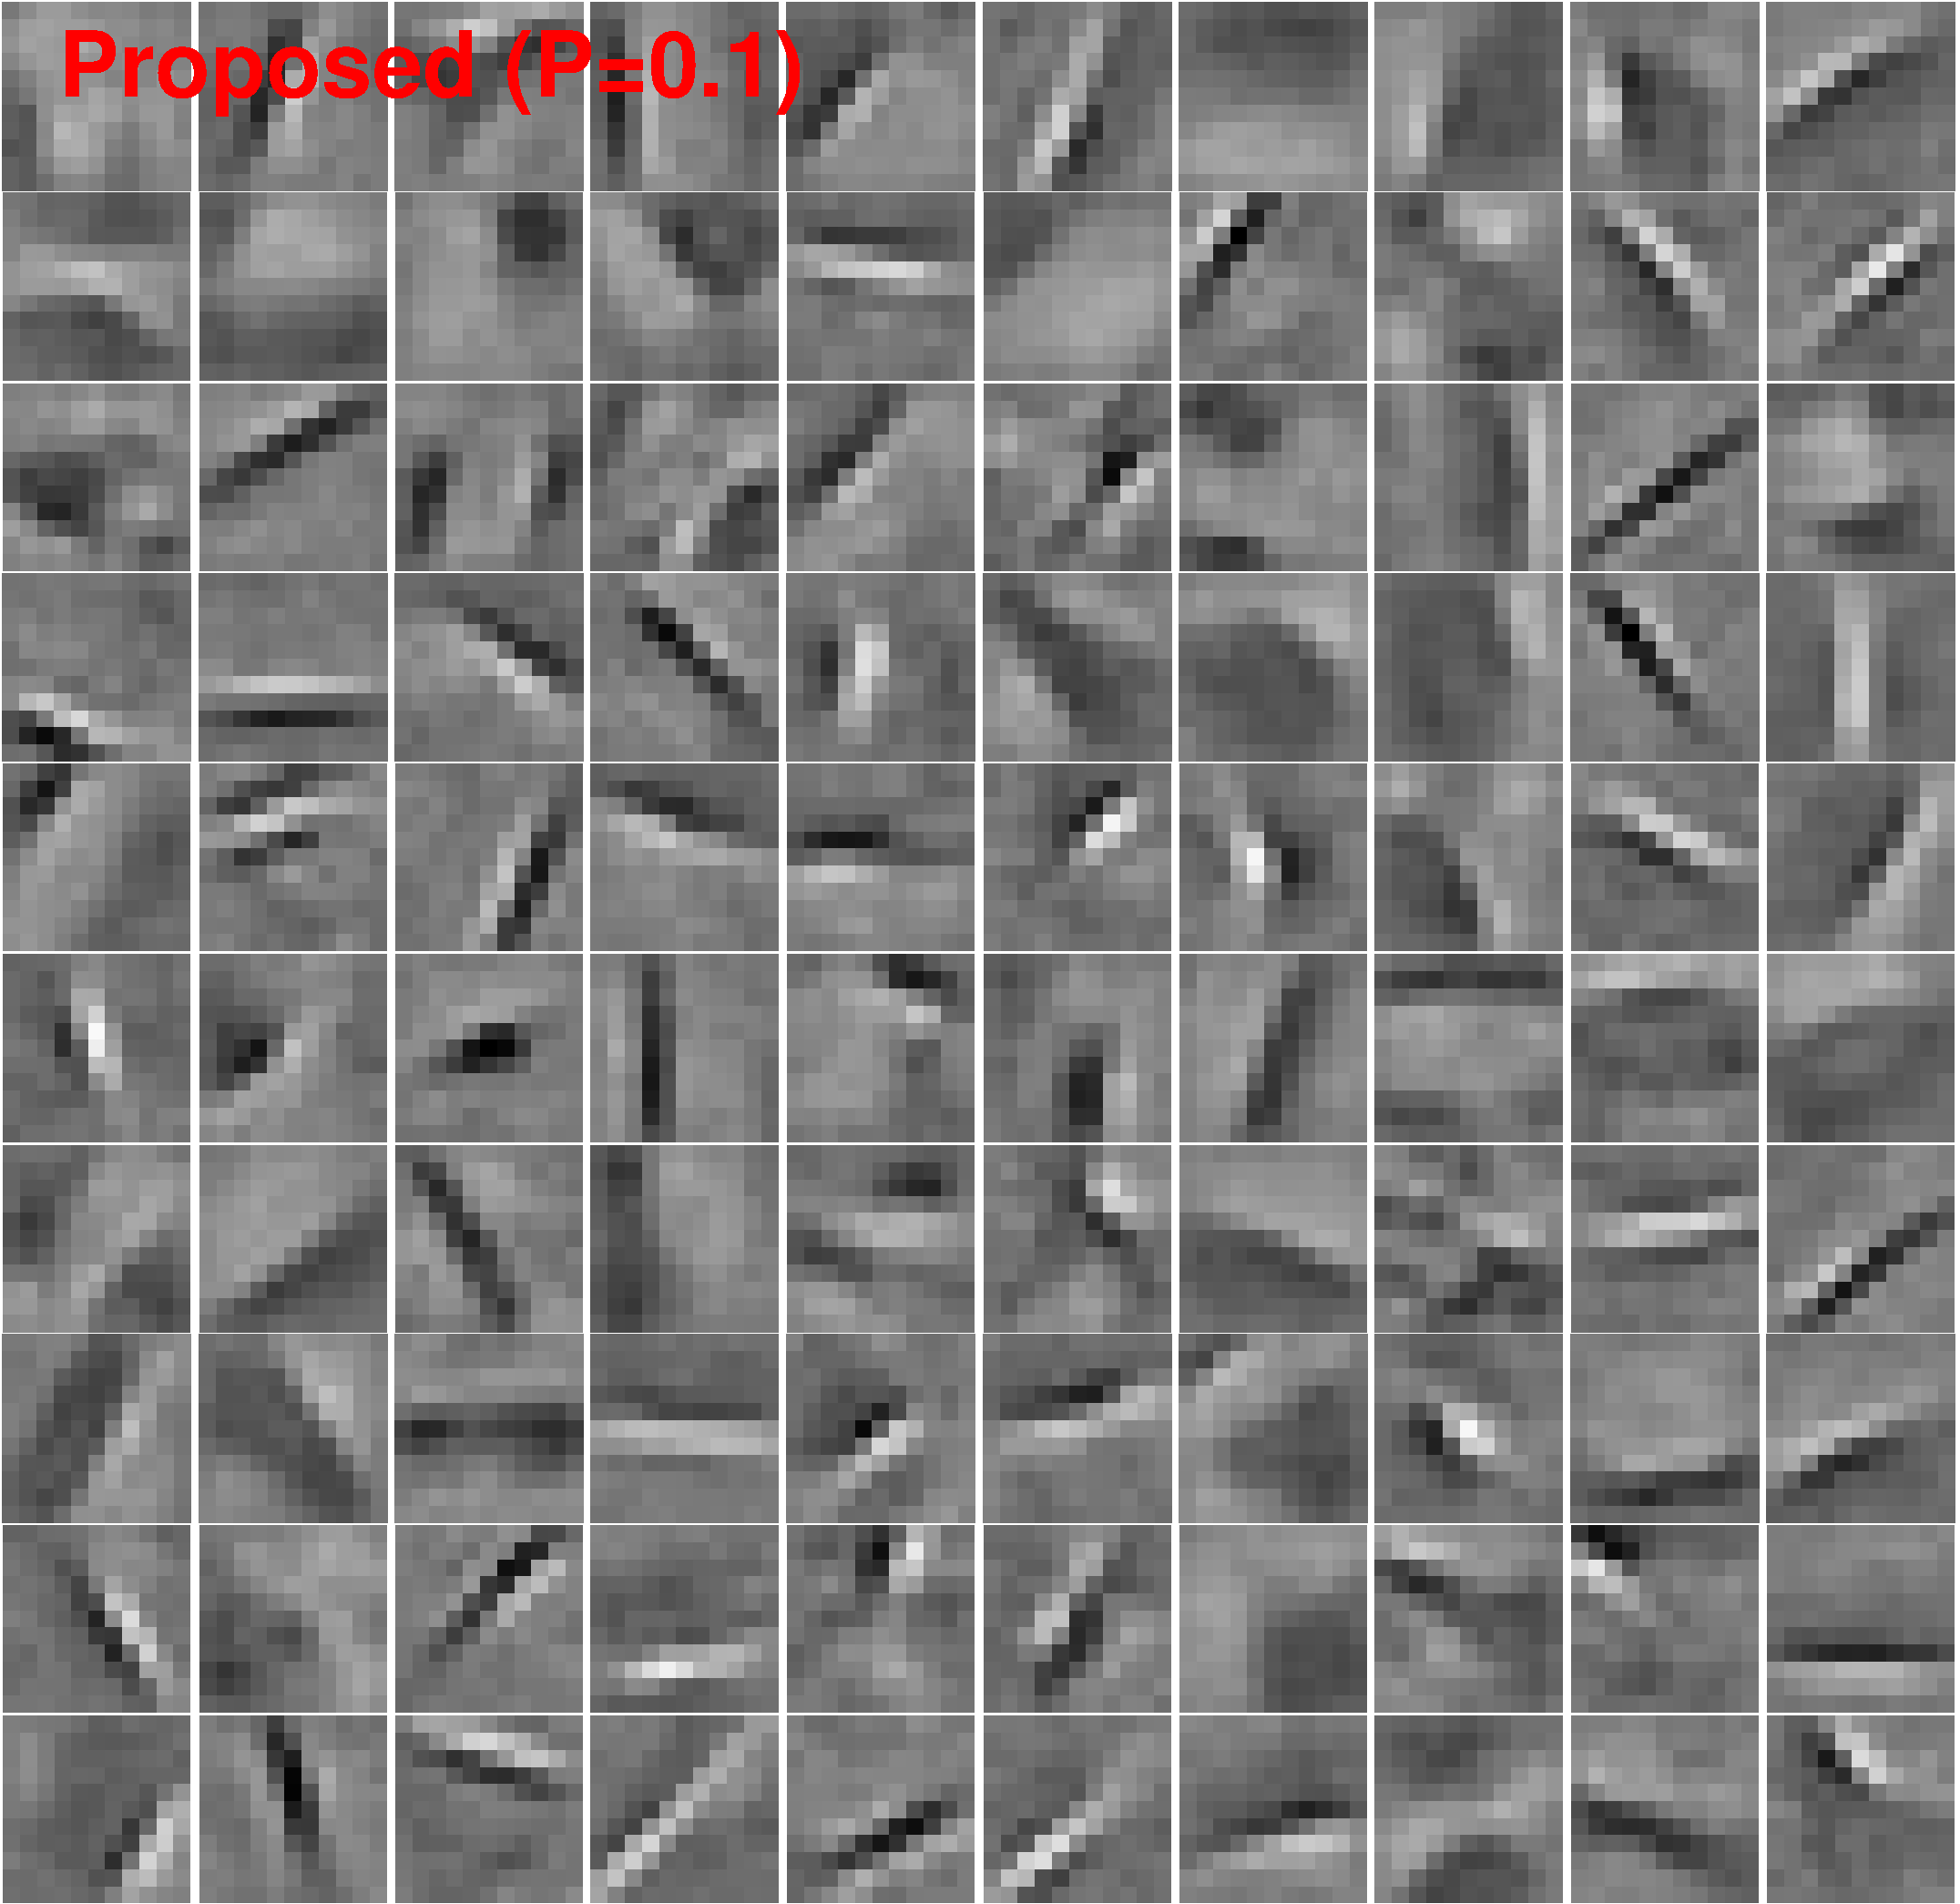
\includegraphics[width=1\linewidth]{figure/batchFruit100.pdf}
\end{subfigure}

\begin{subfigure}{0.6\textwidth}
  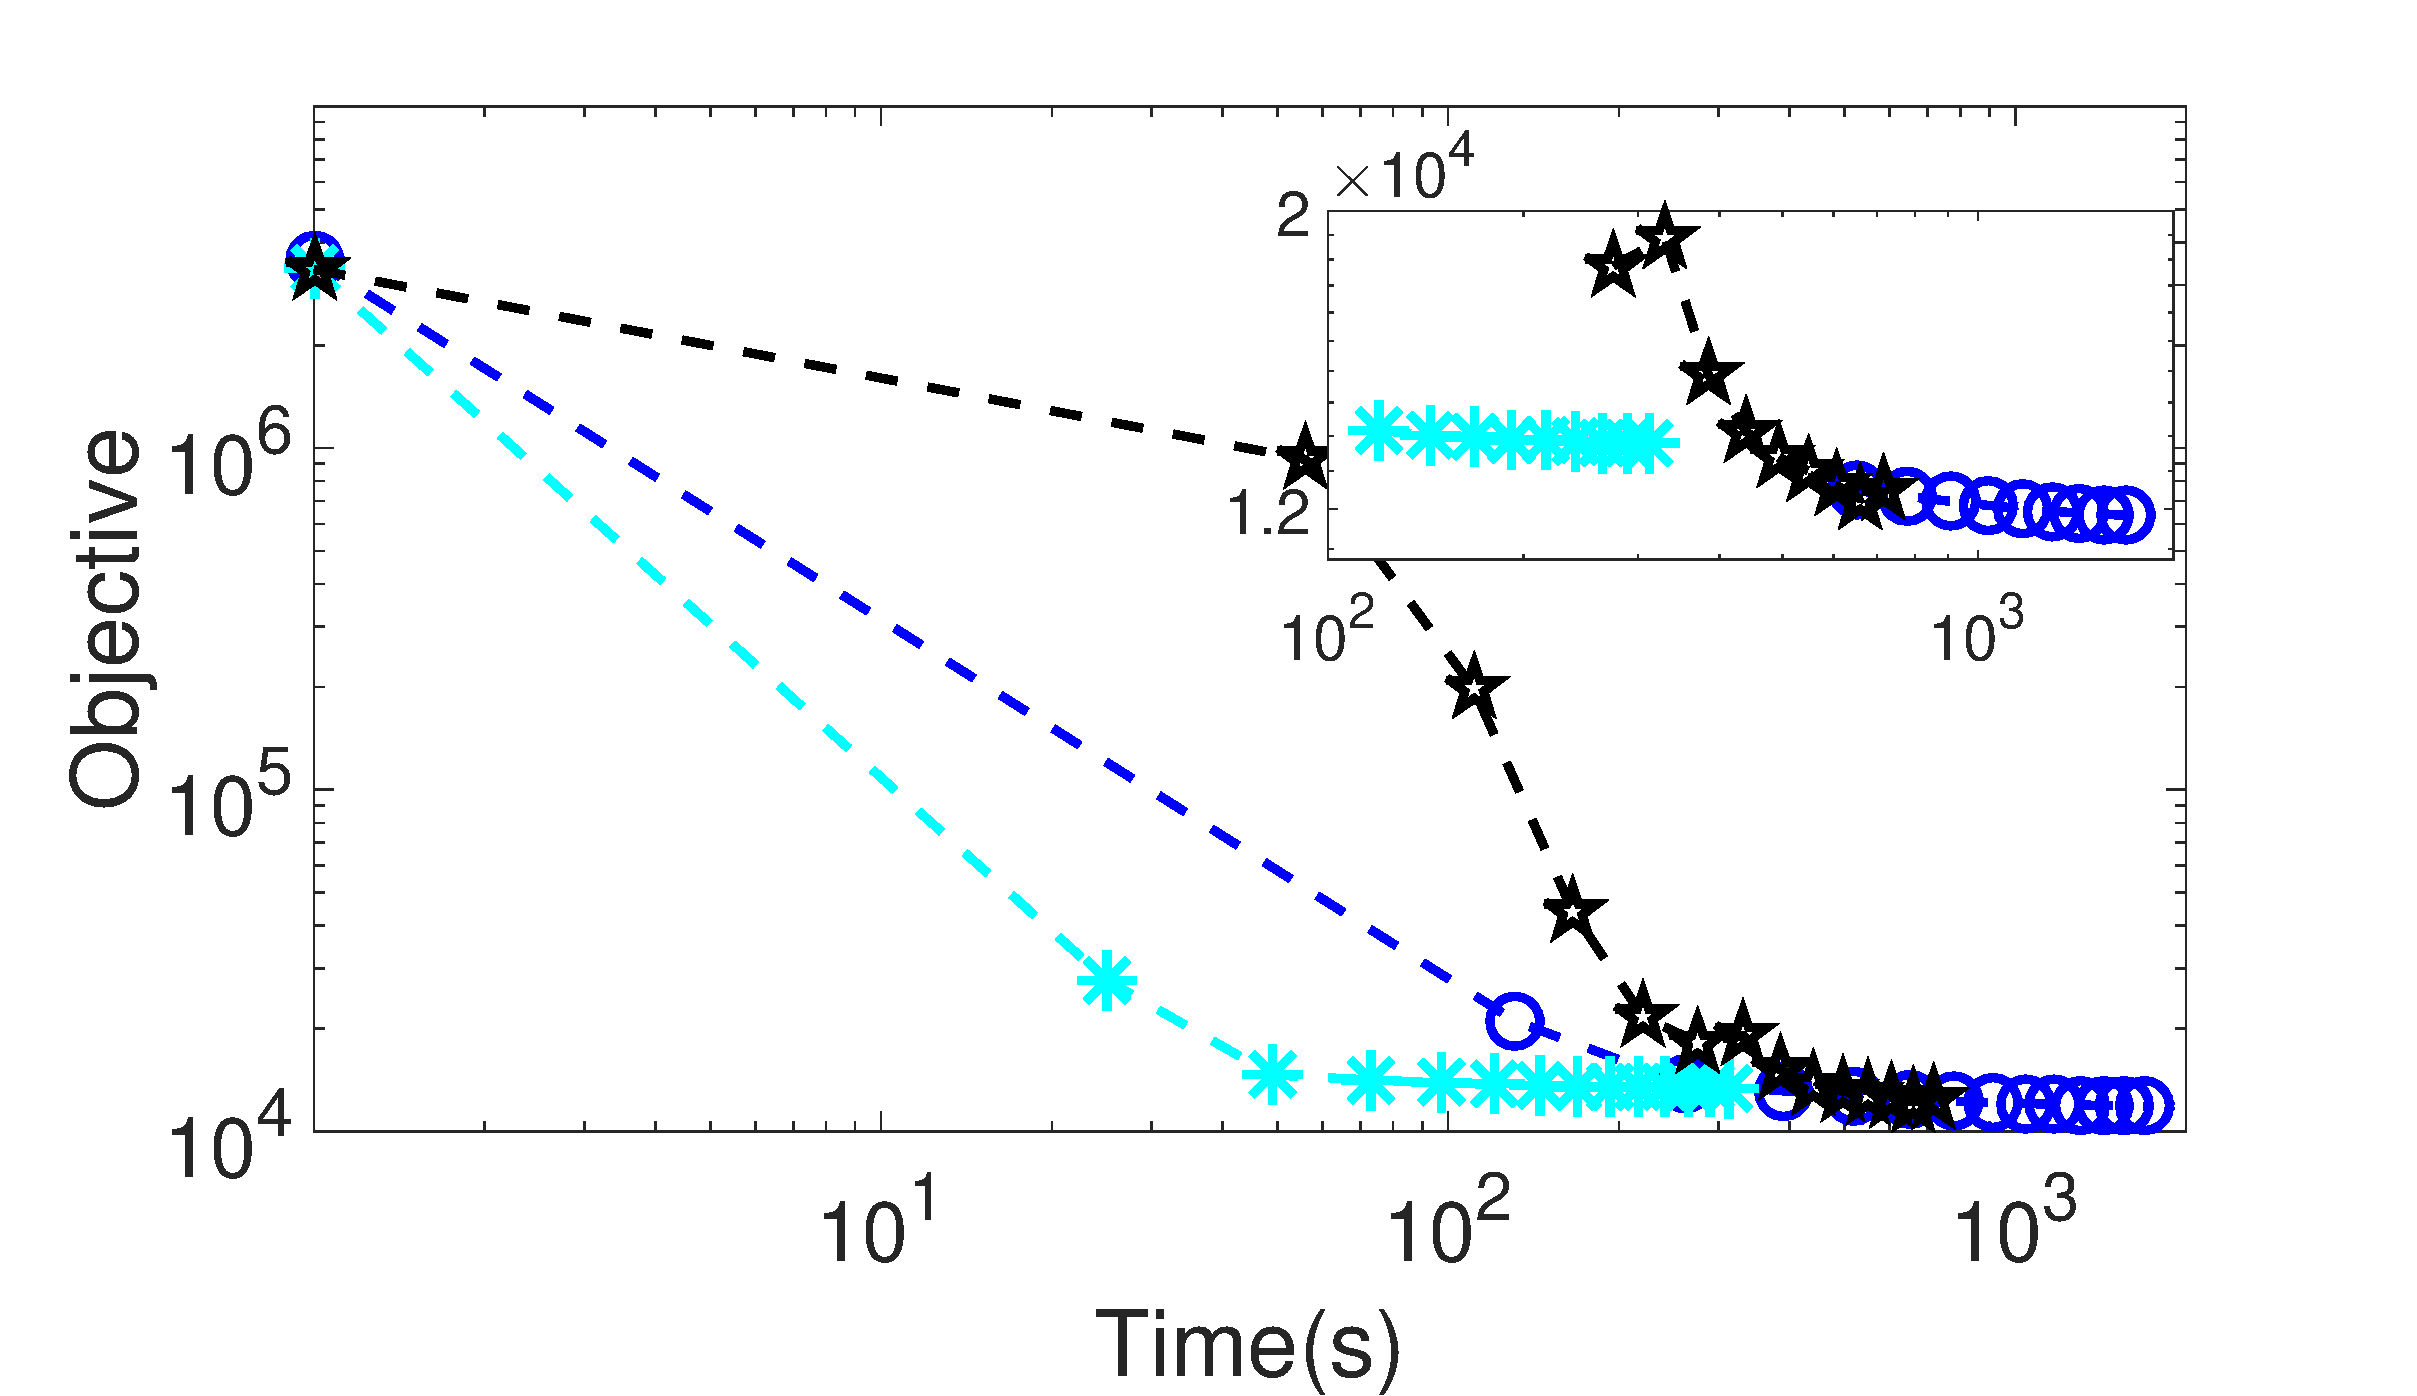
\includegraphics[width=1\linewidth]{figure/timeVSobj.pdf}
\end{subfigure}
\begin{subfigure}{0.3\textwidth}
  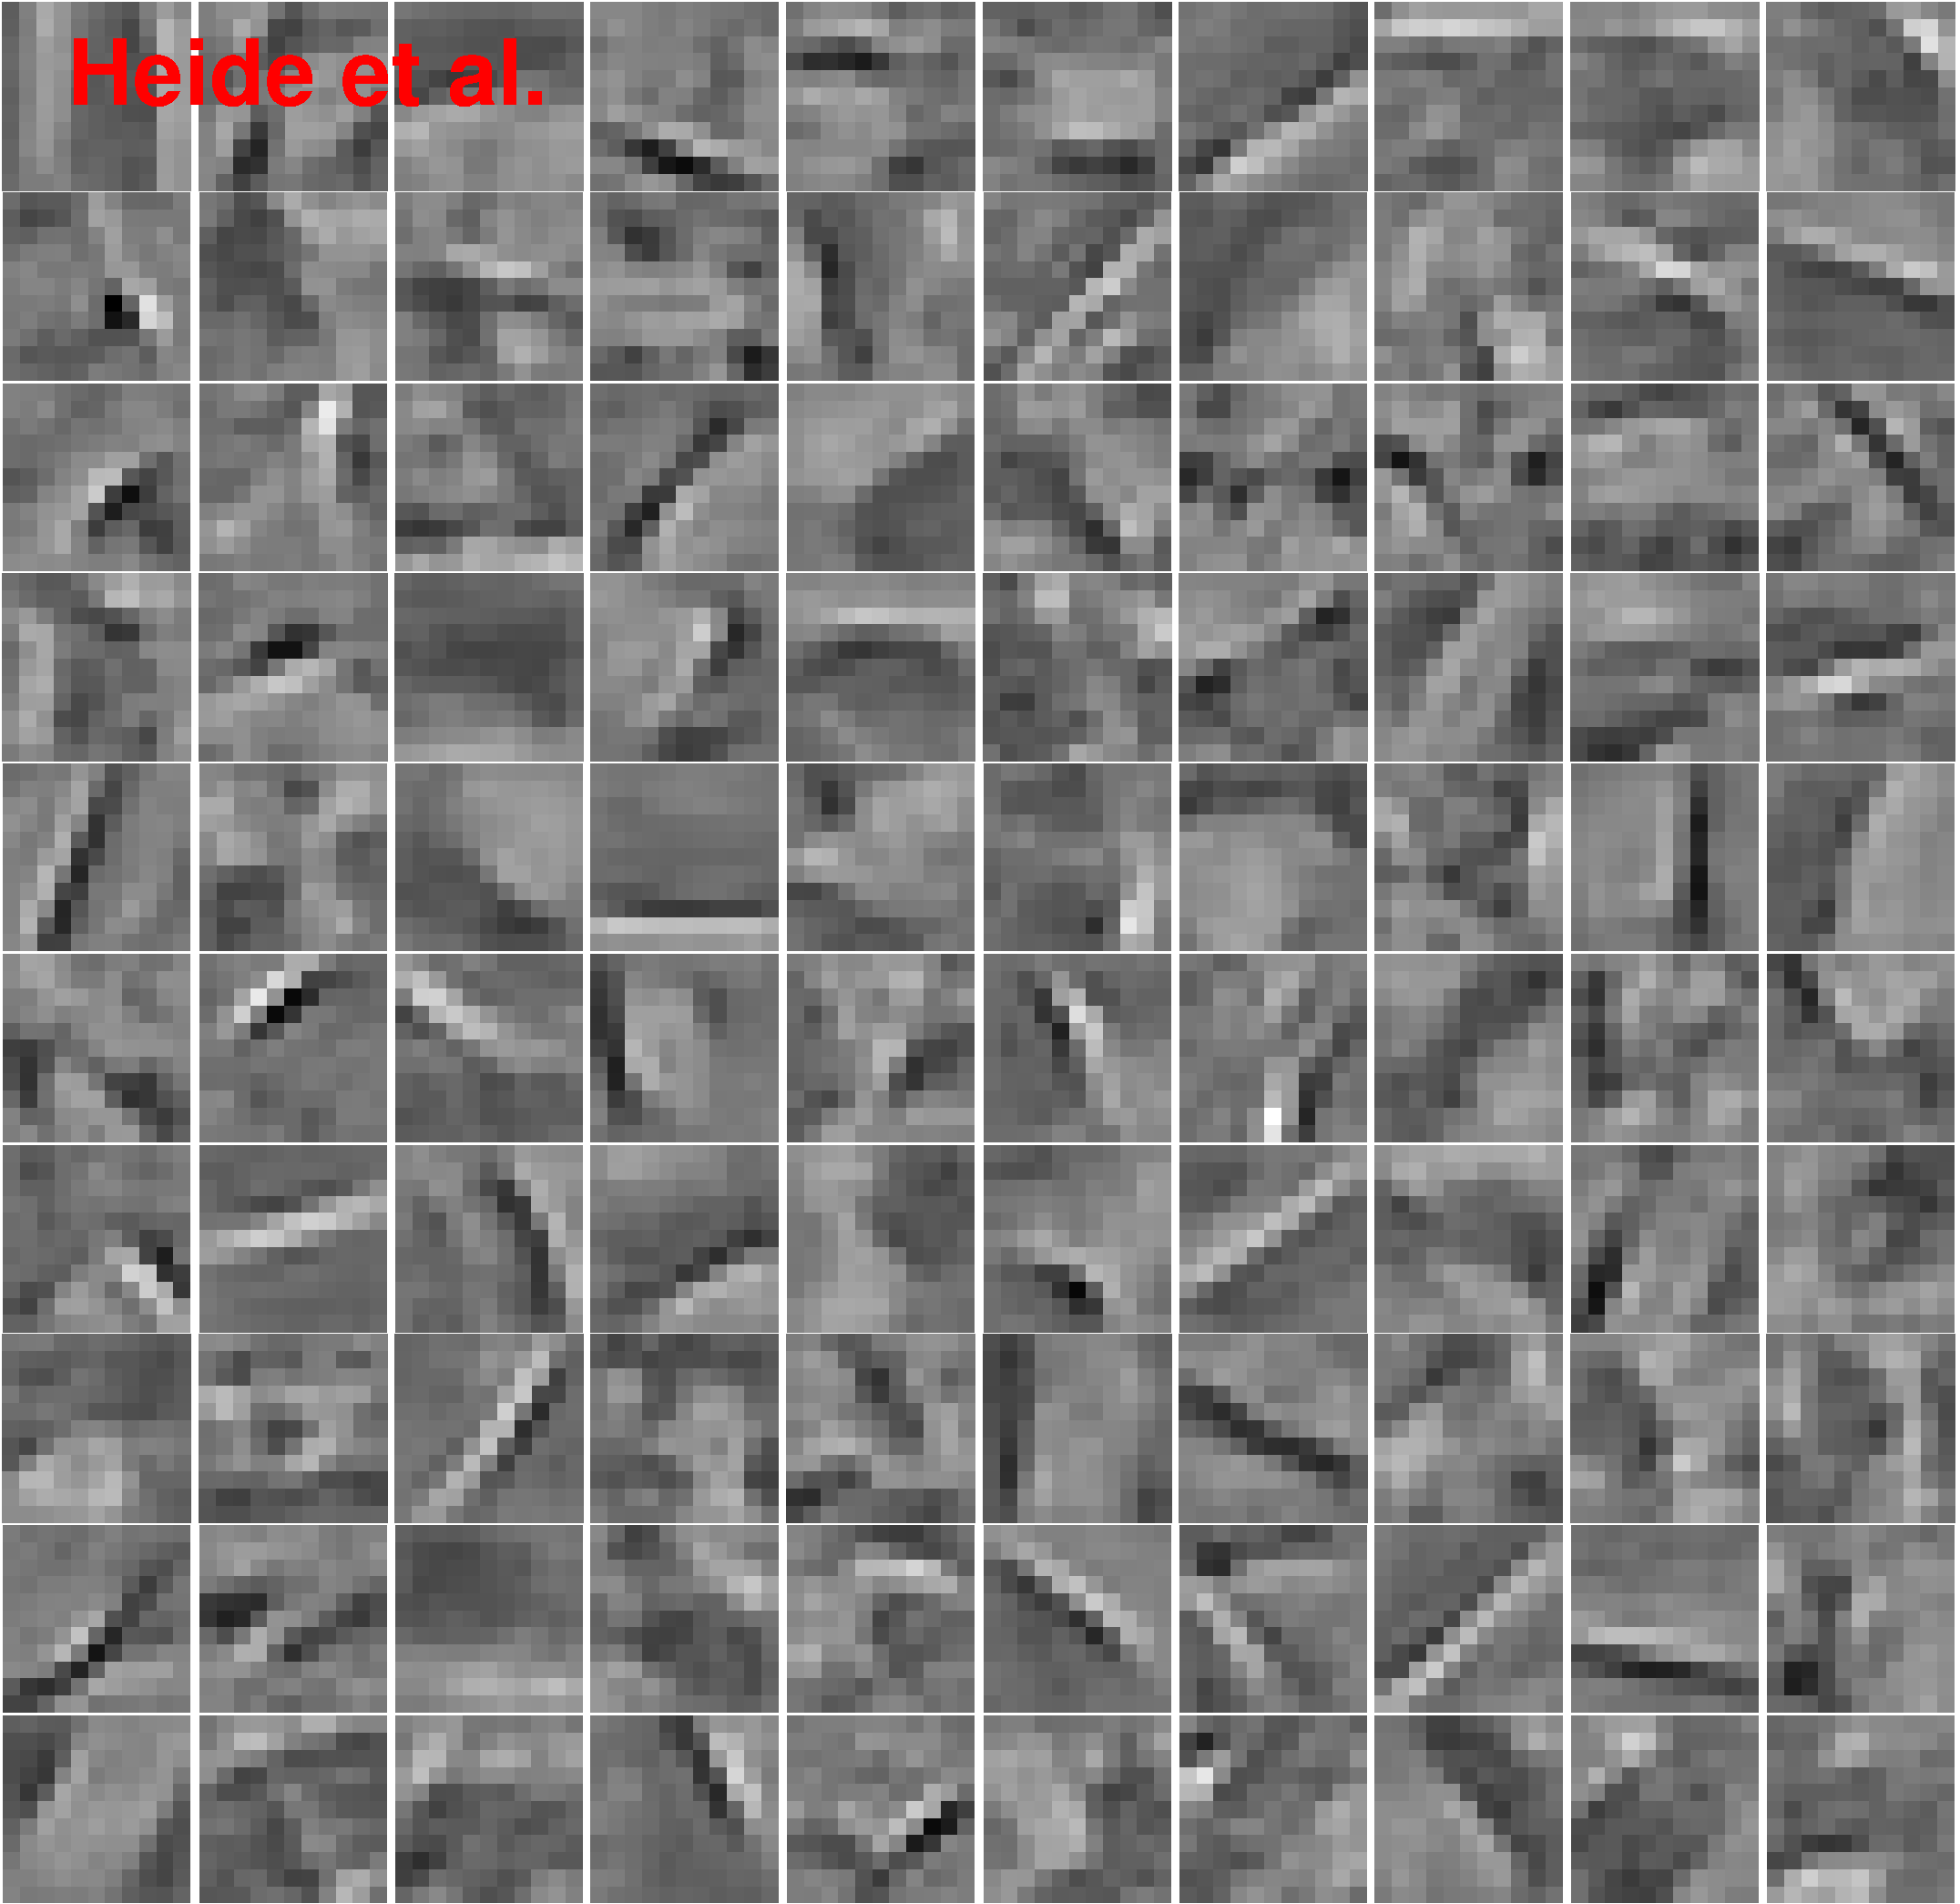
\includegraphics[width=1\linewidth]{figure/heideFruit100.pdf}
\end{subfigure}

\caption{Left: Convergence comparison between the-state-of-art method~\cite{heide2015fast} and the proposed method with different subsampling probability. Right: Learned filters by the proposed method with $p=0.1$ and the comparable method. In these represented learned filters, our method learns more Gabor-like and less noise-like filters. Beyond this, it runs faster with regard to each iteration and shows better convergence behavior.}
\label{fig:subsampleResult}
\end{figure}

{\bfseries Reconstruction}. The learned filters by the proposed method with subsampling rate $0.1$ are shown on the right hand side of Fig.~\ref{fig:subsampleResult}. For a visual comparison, we also show the filters learned from the competing method. As can be observed, both of them learn some seemingly similar Gabor-like filters. While after zooming, it can be seen that our learned Gabor-like filters have less impure structures. Moreover, the comparable filters contain a number of noise-like dictionaries, which are rarely existed in ours. We then demonstrate the effectiveness of the reconstructed filters in the application of image inpainting, which refers to reconstructing a full image from partial measurements. A numerical comparison of the reconstruction quality is shown in Fig.~\ref{fig:PSNRrecon}. The filters learned by the proposed method not only show more visually decent structures and less specific features, but also demonstrate its capability to better reconstruct partial observed images. In addition to that, the learning process only takes about $40\%$ of the execution time of the comparison.

\begin{figure}[h]
    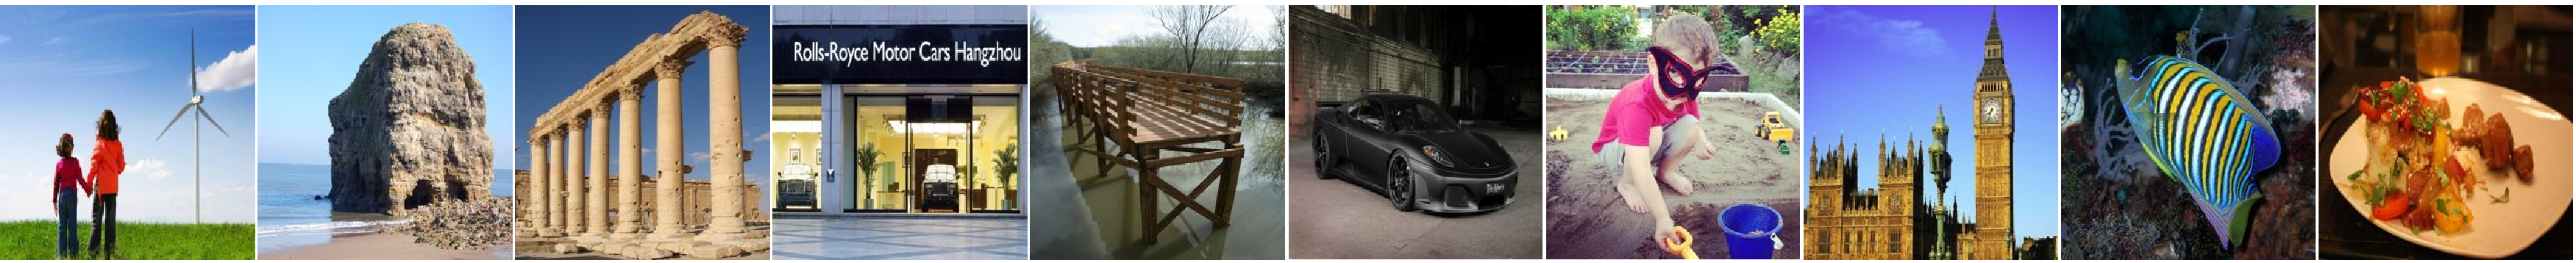
\includegraphics[width=1\textwidth]{figure/reconImage.pdf}
    \\
    \\
    \resizebox{1\linewidth}{!}{
        \begin{tabular}{|c||c|c|c|c|c|c|c|c|c|c|}
            \cline{1-11}
            Image & 1 & 2 & 3 & 4 & 5 & 6 & 7 & 8 & 9 & 10 \\
            \hline
            PSNR~\cite{heide2015fast} & 29.54 & 28.16 & 29.40 & 29.22 & 28.89 & 29.29 & 28.10  & 29.57 & 27.46 & 30.72 \\
            \hline
            PSNR ours & \textbf{29.65} & \textbf{28.18} & \textbf{29.52} & \textbf{29.43} & \textbf{28.99} & \textbf{29.38} & \textbf{28.19} & \textbf{29.63} & \textbf{27.62} & \textbf{30.98} \\
            \hline
        \end{tabular} }
    \caption{Numerical comparisons of the reconstruction quality obtained from the presented filters and its comparison. The reconstructions are performed on $50\%$ randomly observed images, with $\lambda = 0.4$ and $50$ ADMM iterations for both cases. Obtained PSNR values are averaged on 5 trials. Note that none of the testing images are in the training sets.} \label{fig:PSNRrecon}
\end{figure}

\subsection{Online Learning Settings}
We further evaluate the online fashion of the proposed method. To begin with, we validate the proposed algorithm on the city dataset~\citep{zeiler2010deconvolutional}, which has 10 training images and 4 testing images, and all of them has the size of $100 \times 100$. Afterwards, we analyze the effectiveness of over-complete dictionary learned from 1000 images randomly picked up from ImageNet~\cite{deng2009imagenet}.

{\bfseries Convergence.} Unlike the batch-based learning approaches, the training loss objective of the entire dataset cannot be evaluated since each training step only draws one or a few of the data samples. Nevertheless, we can evaluate the learning process on testing images. The loss objectives on testing dataset of the proposed online learning algorithm and prior published online CSC model solved in frequency domain~\citep{liu-2018-first}, with respect to iterations, are shown in Fig.~\ref{fig:onlineSmall}. In the same figure, we also keep track of the capability of the updated filters in the learning process to sparsely represent the testing images, which are demonstrated by its PSNR with respect to time. These two approaches stop at optimum positions with close testing objective values, though, they exhibit slightly different convergence behaviors with respect to iterations. The final testing PSNR values for both methods also reveal the similar reconstruction performance of the learned filters. As for the runtime comparison, the proposed method runs at least 5 times faster than its comparative.

%The proposed method not only exhibits a better convergence performance, but also takes much less execution time, achieving roughly $5 \times$ speedup for one iteration. A visual comparison of the learned dictionaries also demonstrates that the proposed algorithm delivers better outcomes. 
% Further numerical comparison will be reported in the next section.

\begin{figure}[h]
\centering
\begin{subfigure}{0.45\textwidth}
  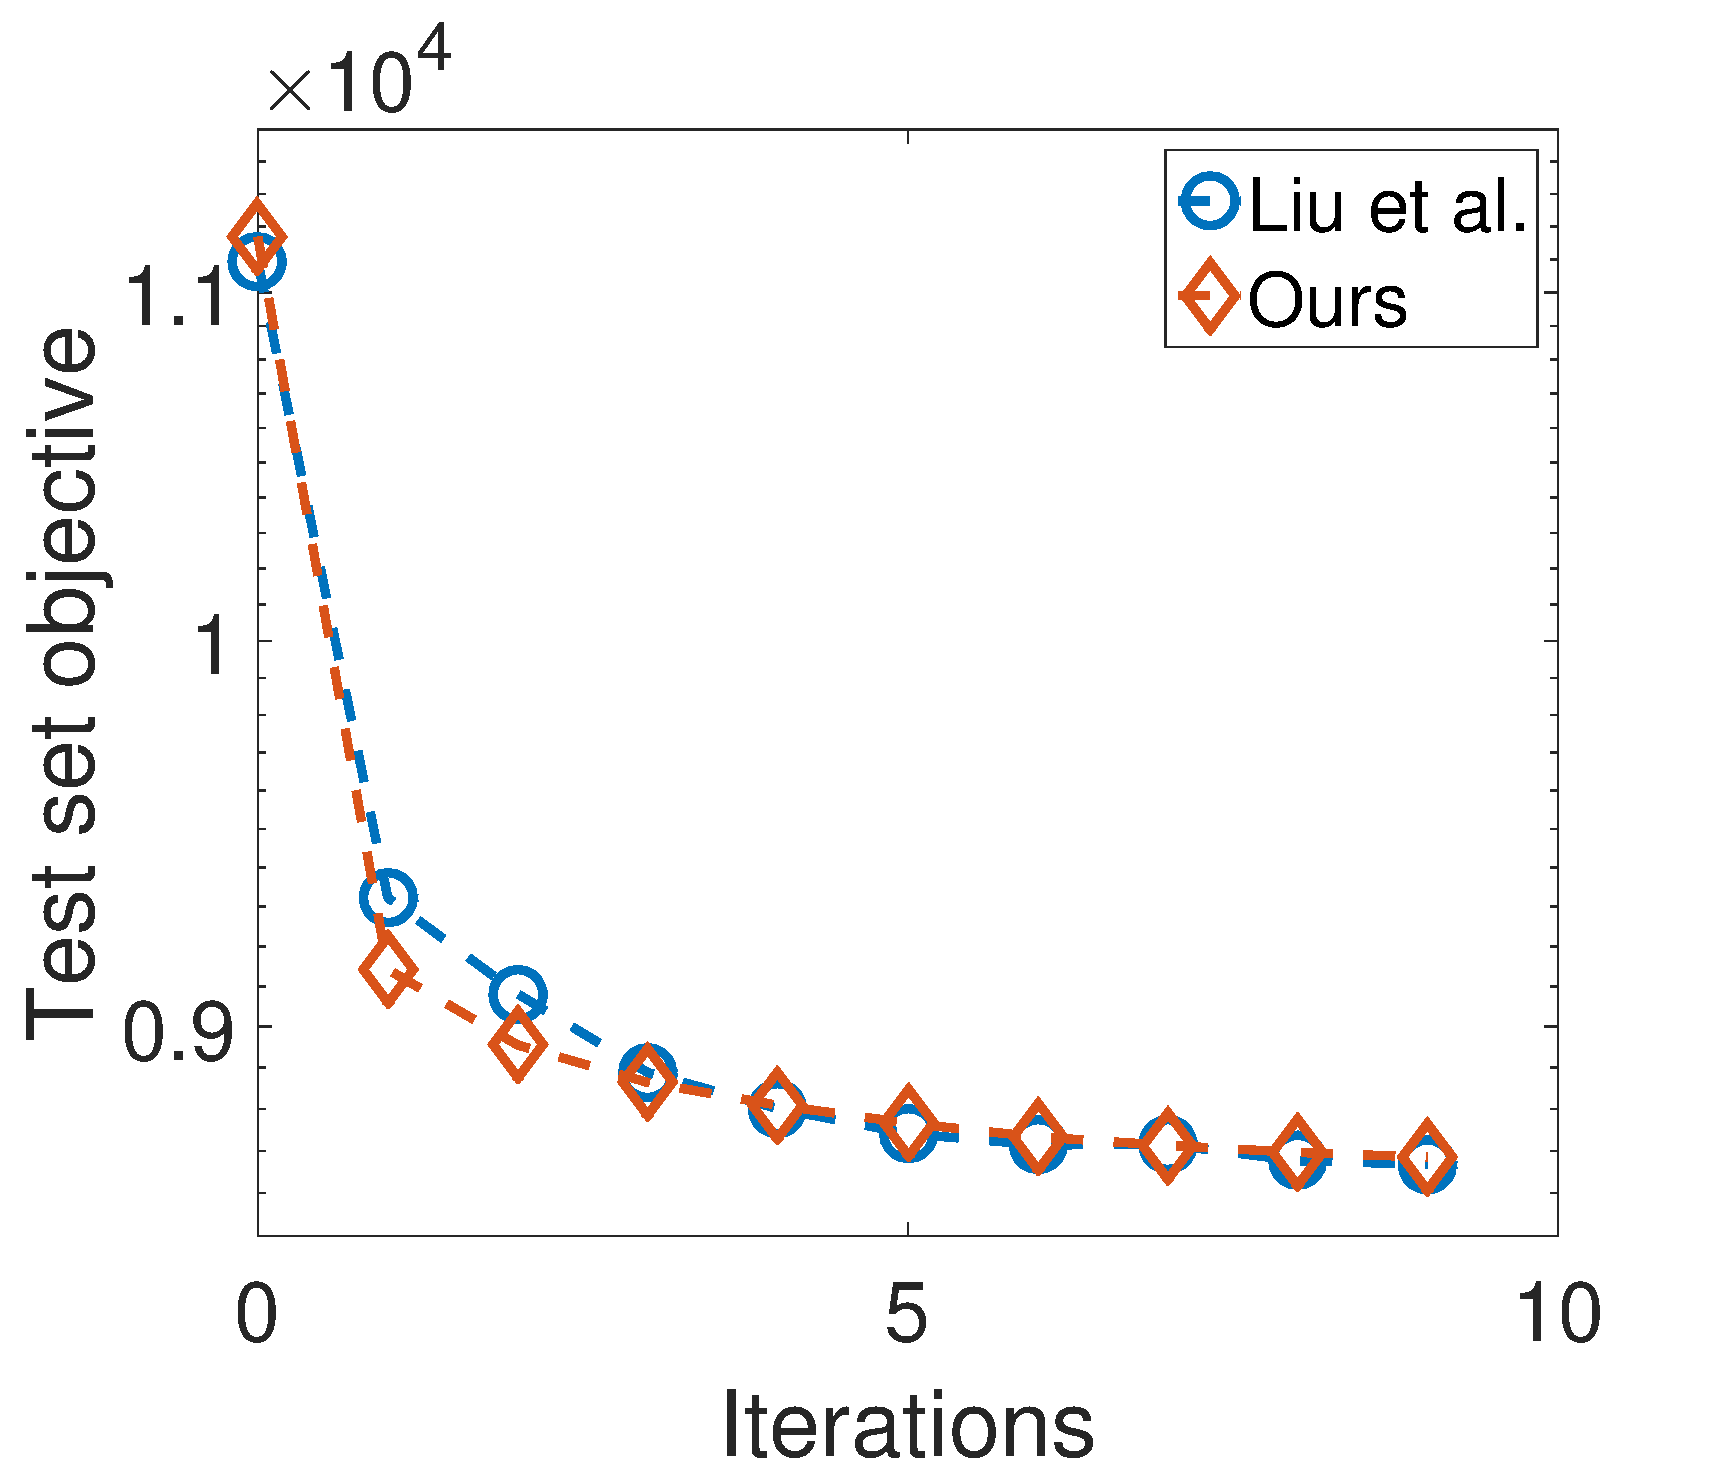
\includegraphics[width=1\linewidth]{figure/onlineVSliu-ite.pdf}
\end{subfigure} 
\begin{subfigure}{0.45\textwidth}
  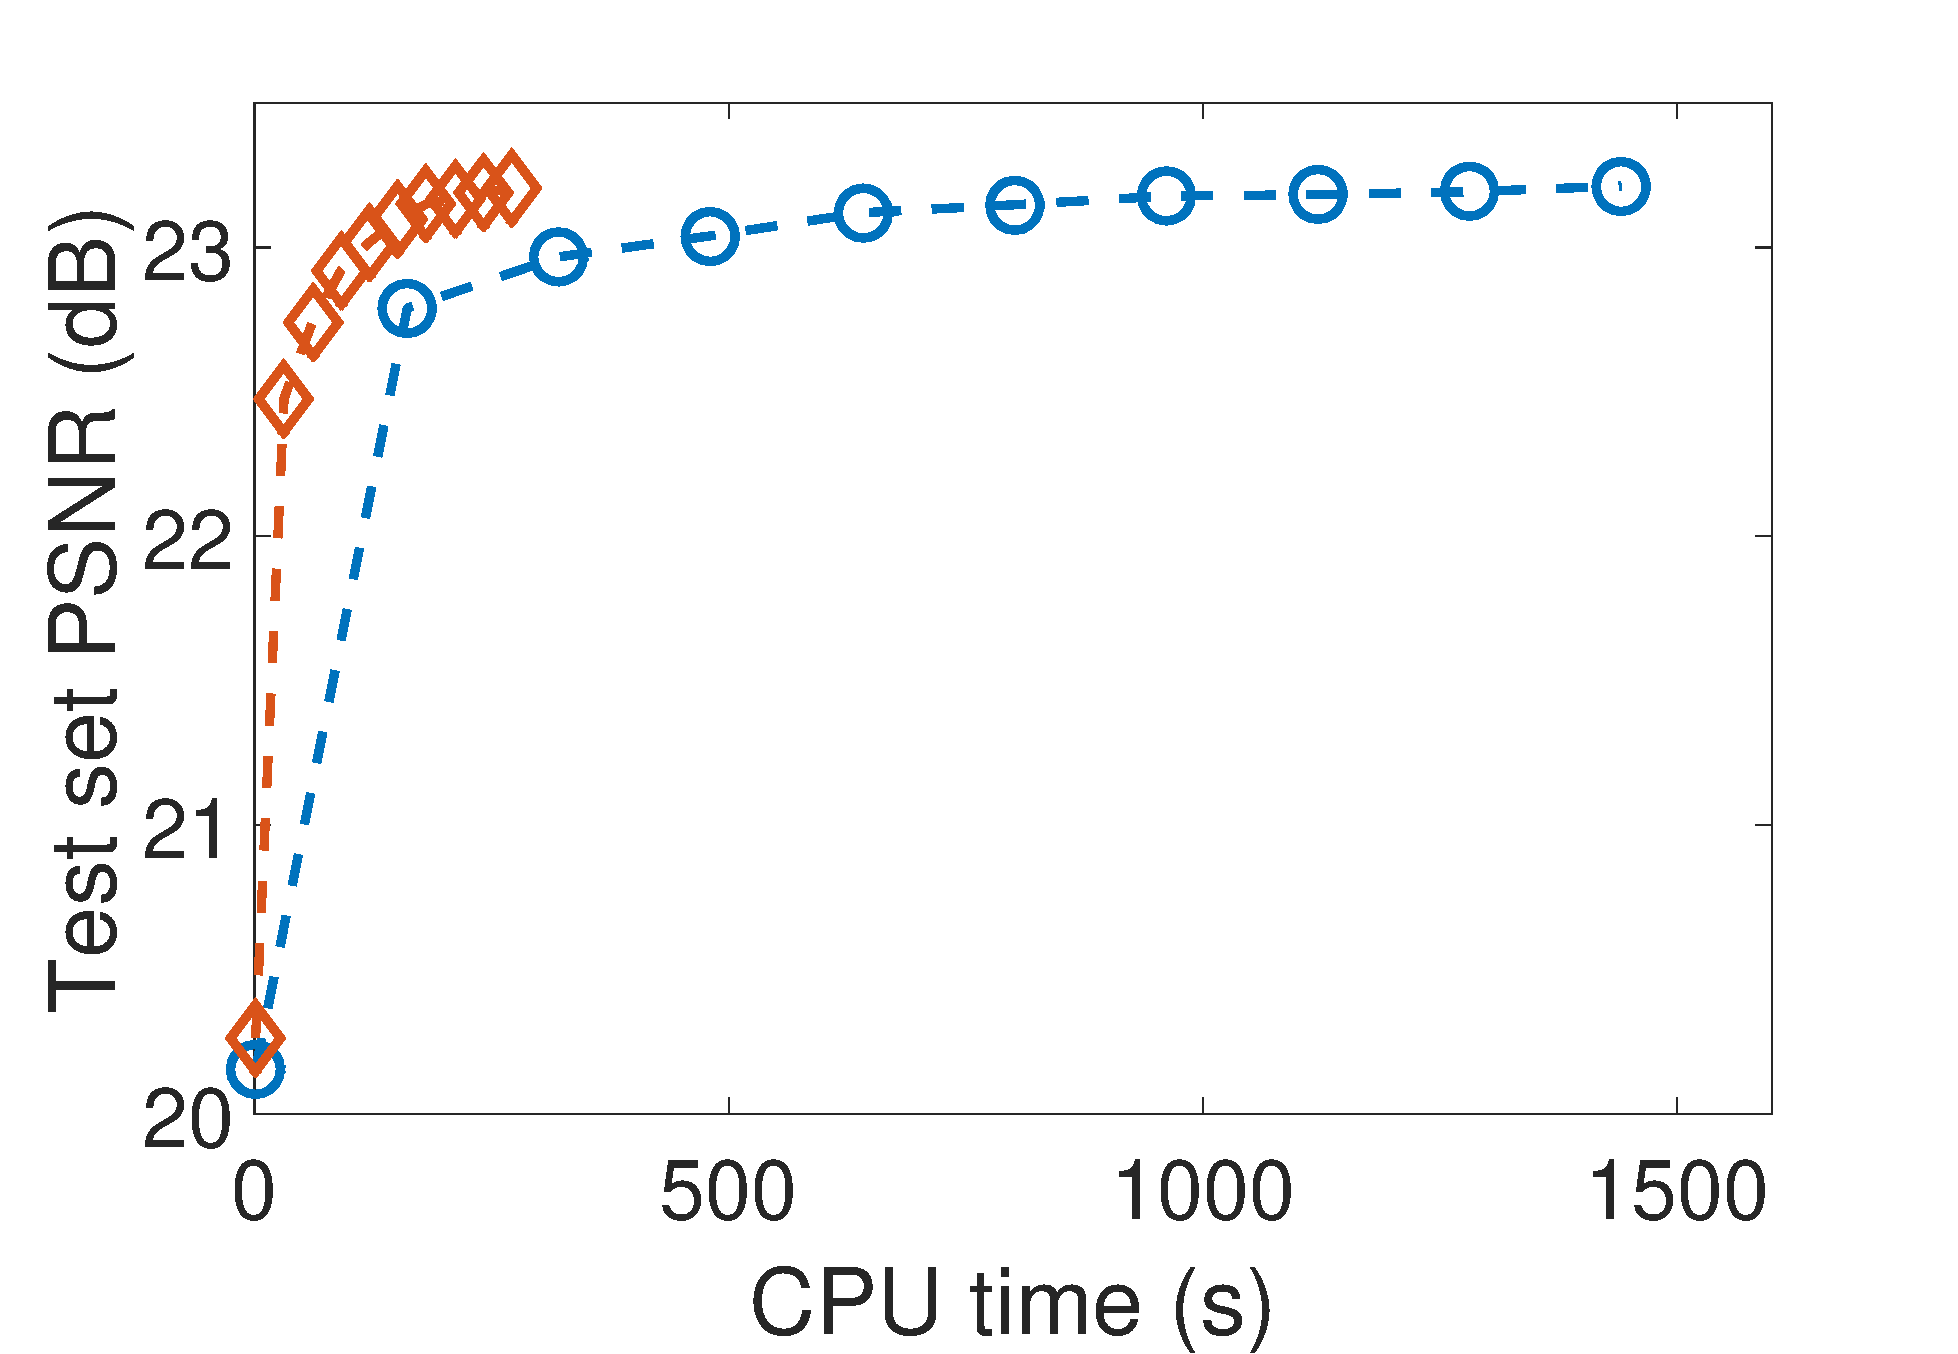
\includegraphics[width=1\linewidth]{figure/onlineVSliu-time.pdf}
\end{subfigure}

\caption{Left: Convergence of the test set objectives for our method (SOCSC) and the state-of-the-art approach~\cite{liu-2018-first}. Right: Testing PSNR with respect to execution time. While the quality of the output is comparable, our method achieves $5 \times$ speedup. \peter{Are the colors correct? The other method seems to be better!}}
\label{fig:onlineSmall}
\end{figure}

{\bfseries Over-complete dictionaries.} As far as we know, none of the precedent CSC work reported or analyzed the over-complete dictionary (the number of filters is more than the degrees of freedom). One of the reasons could be that most of the prior work is batch-based approach, thus learning over-complete dictionary from small dataset would cause the overfitting issue, which may contain quite a few data-specific filters, and therefore be short of the generalization ability. The proposed online-based learning strategy can overcome this issue by scaling up to arbitrary sample sizes.

\begin{figure}[h]
\begin{minipage}{0.4\textwidth}
\begin{subfigure}{1\textwidth}
    \centering
  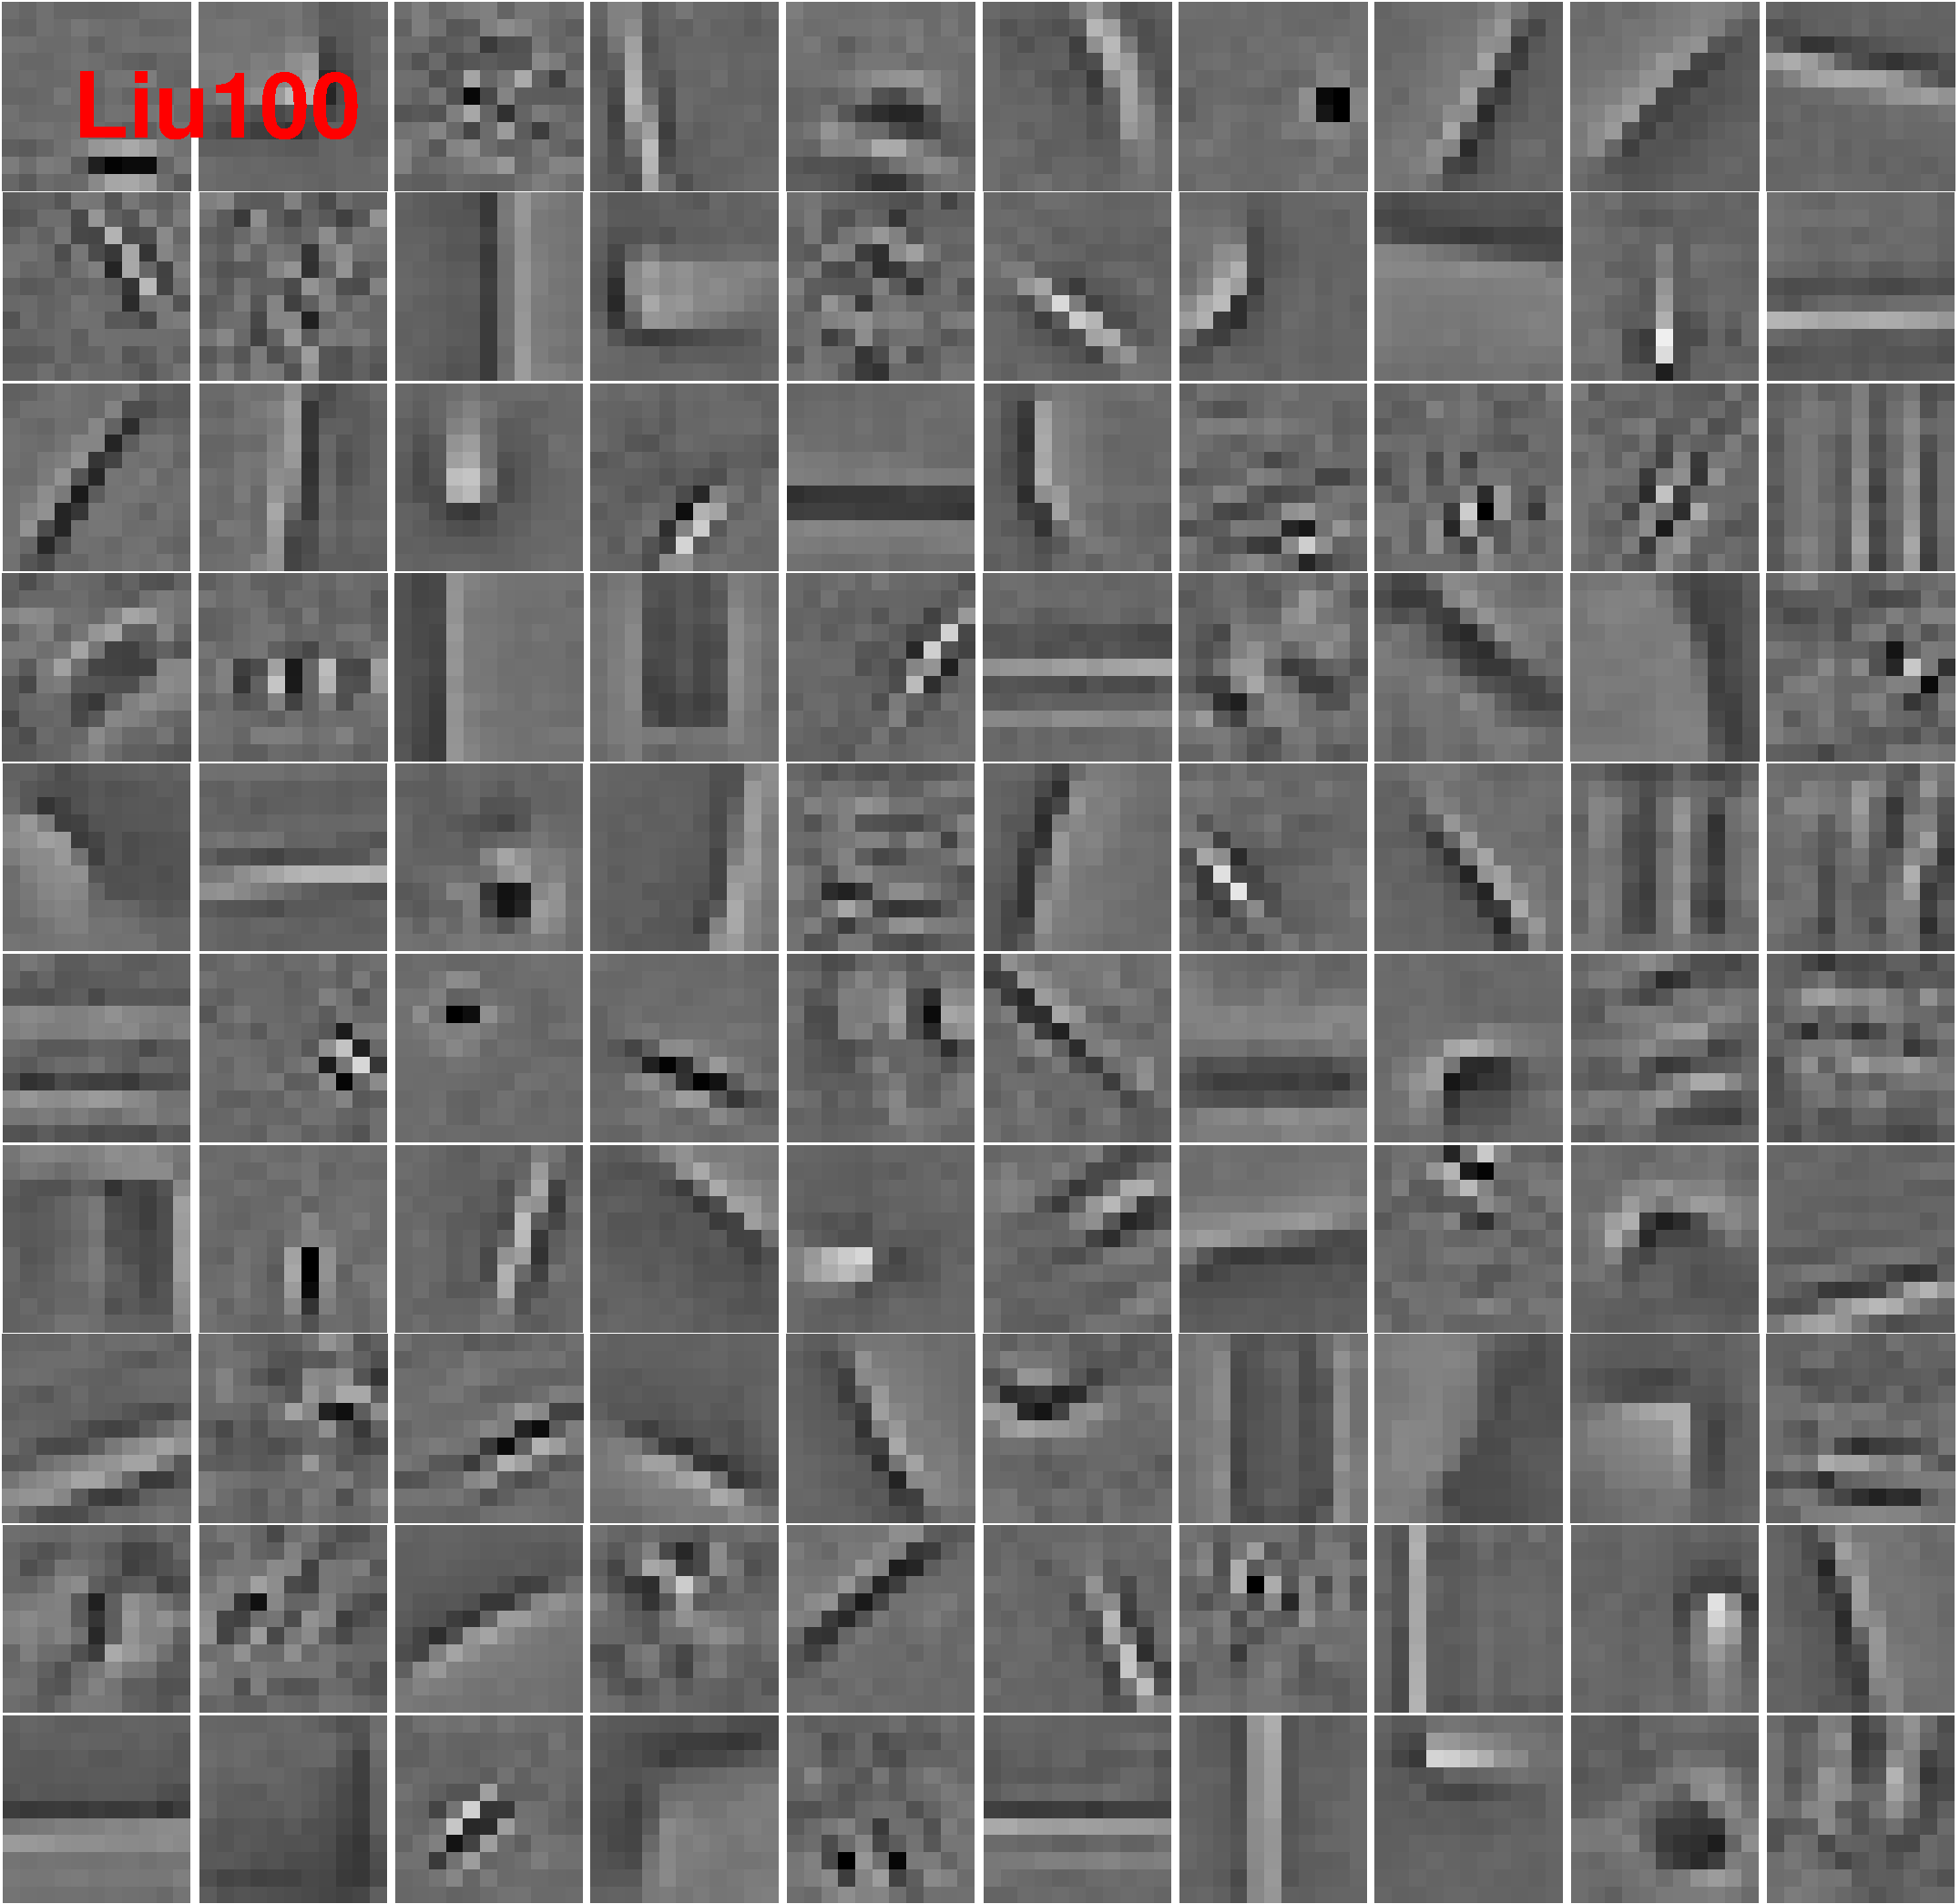
\includegraphics[width=0.6\linewidth]{figure/liu100-filter.pdf}
  \vspace*{2mm}
\end{subfigure}

\begin{subfigure}{1\textwidth}
    \centering
  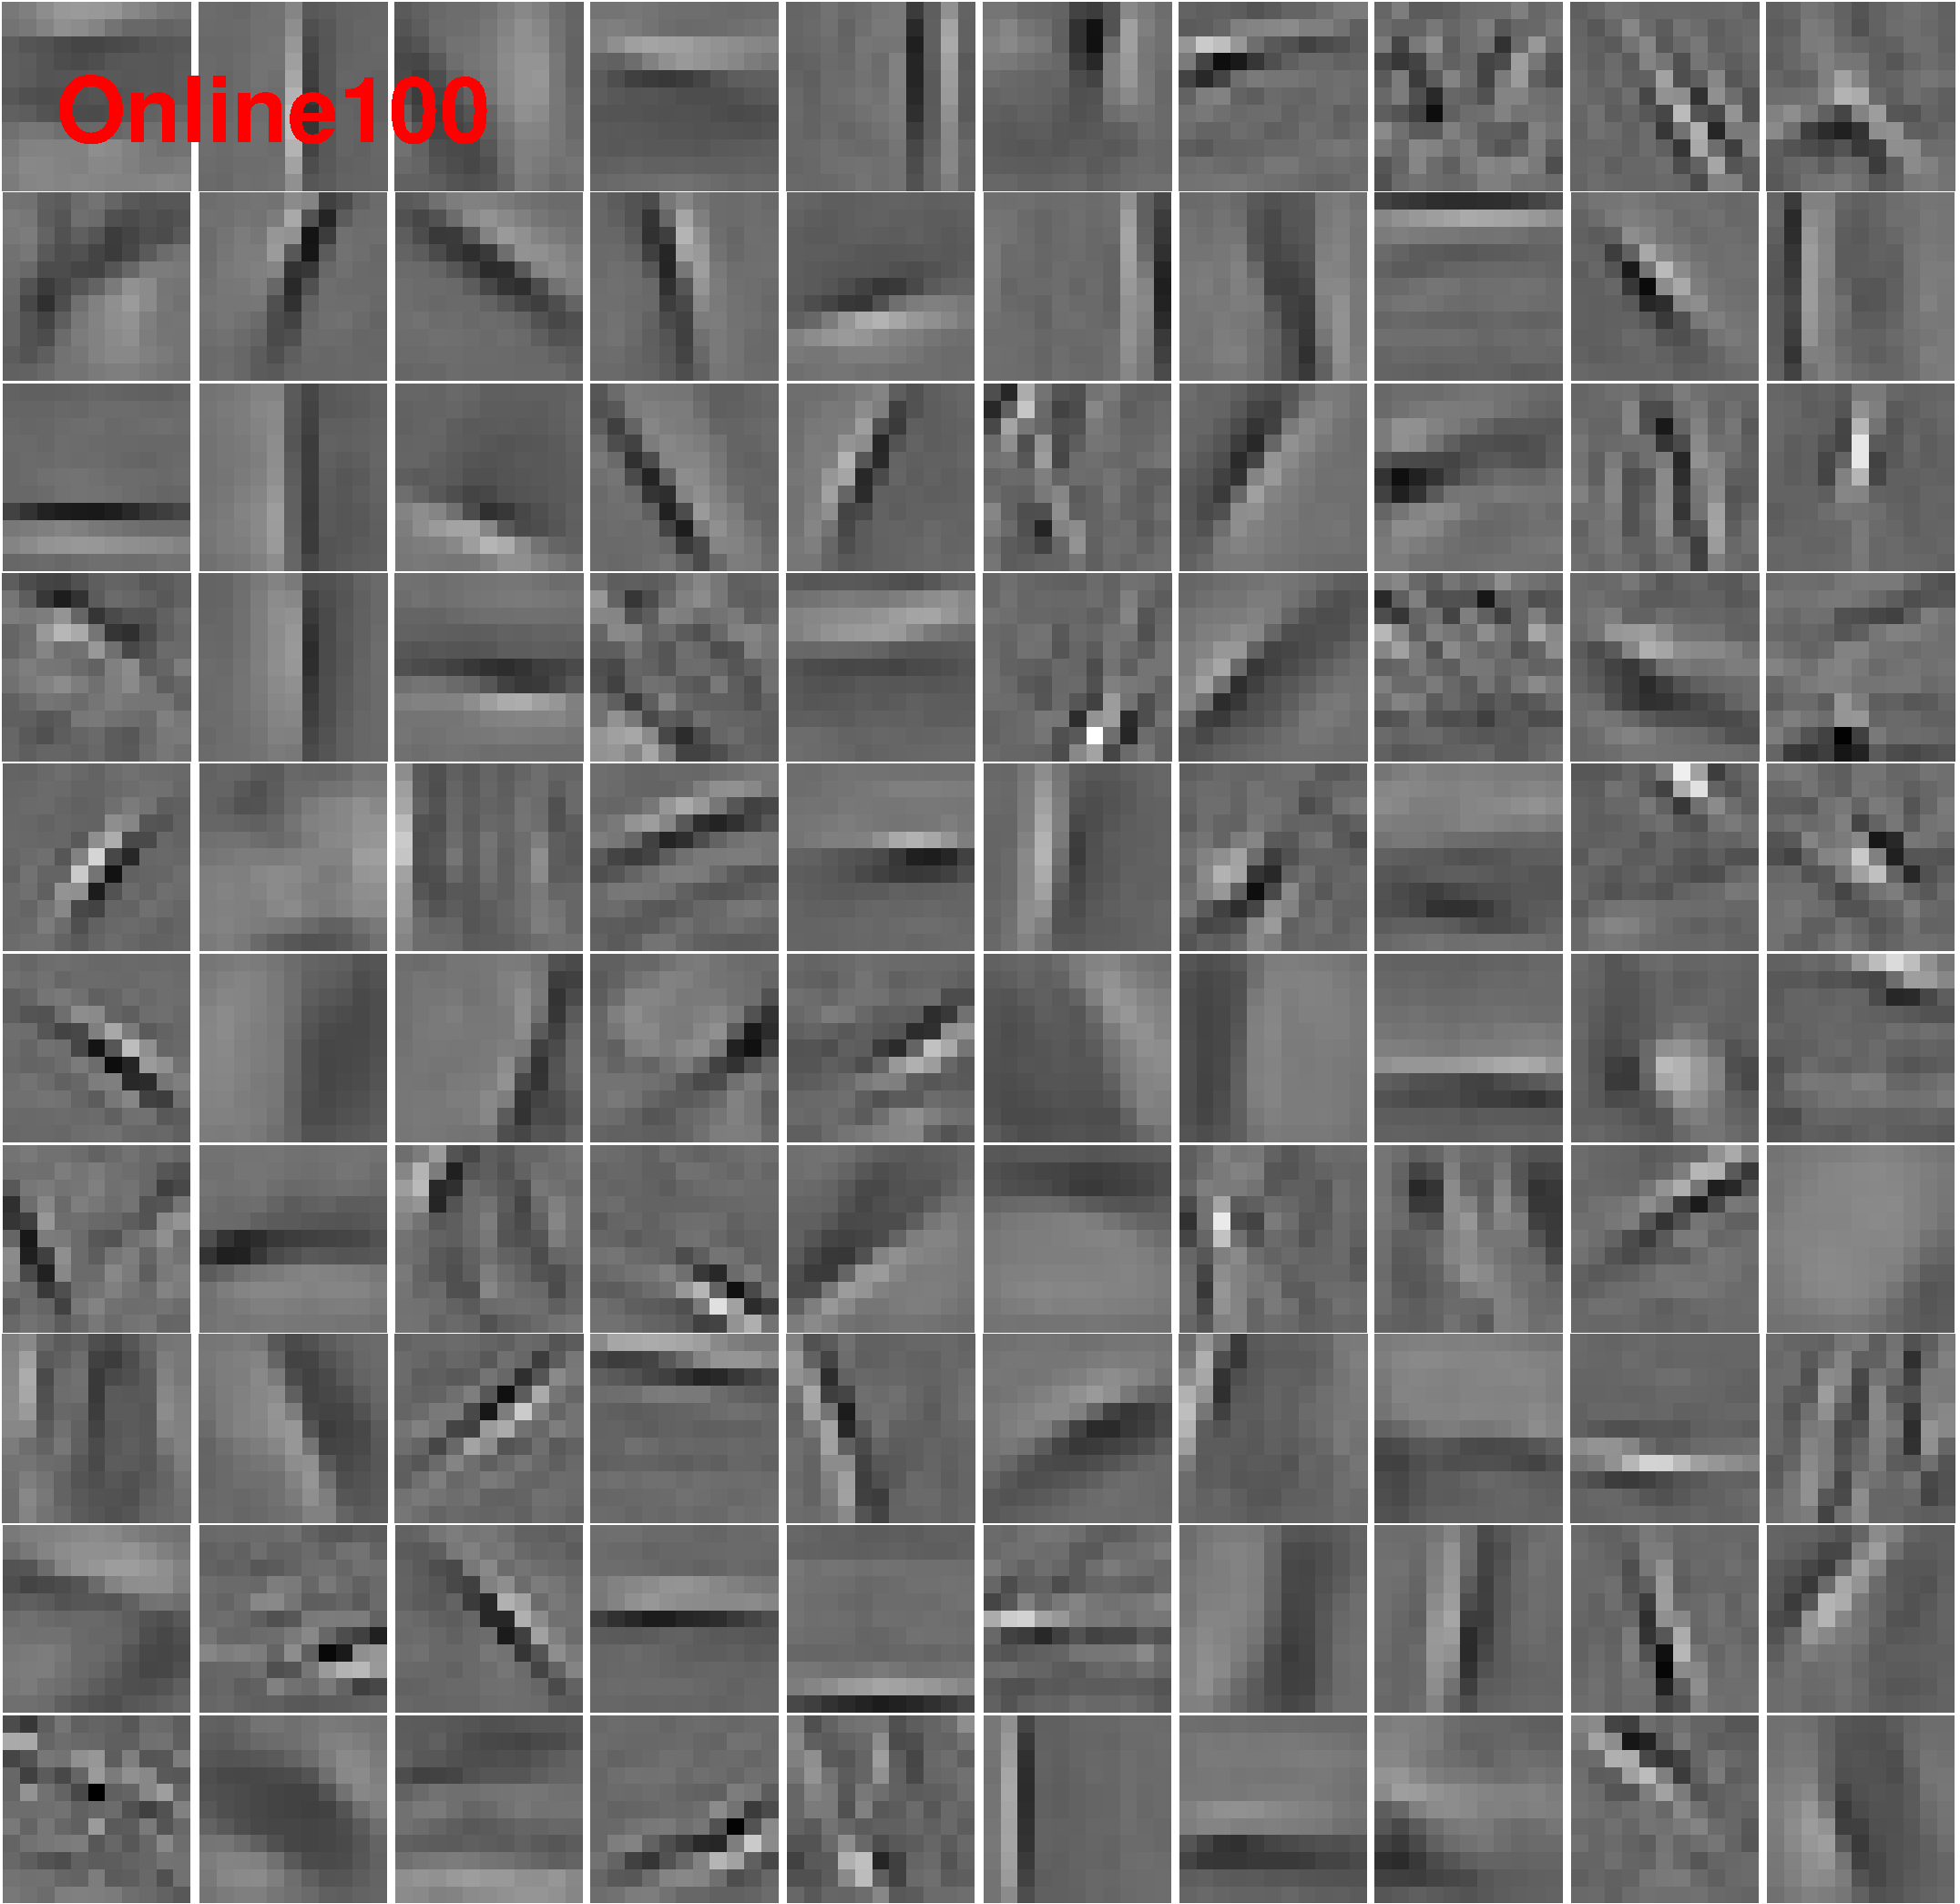
\includegraphics[width=0.6\linewidth]{figure/online100-filter.pdf}
\end{subfigure}
\end{minipage}
\begin{minipage}{0.5\textwidth}
\centering
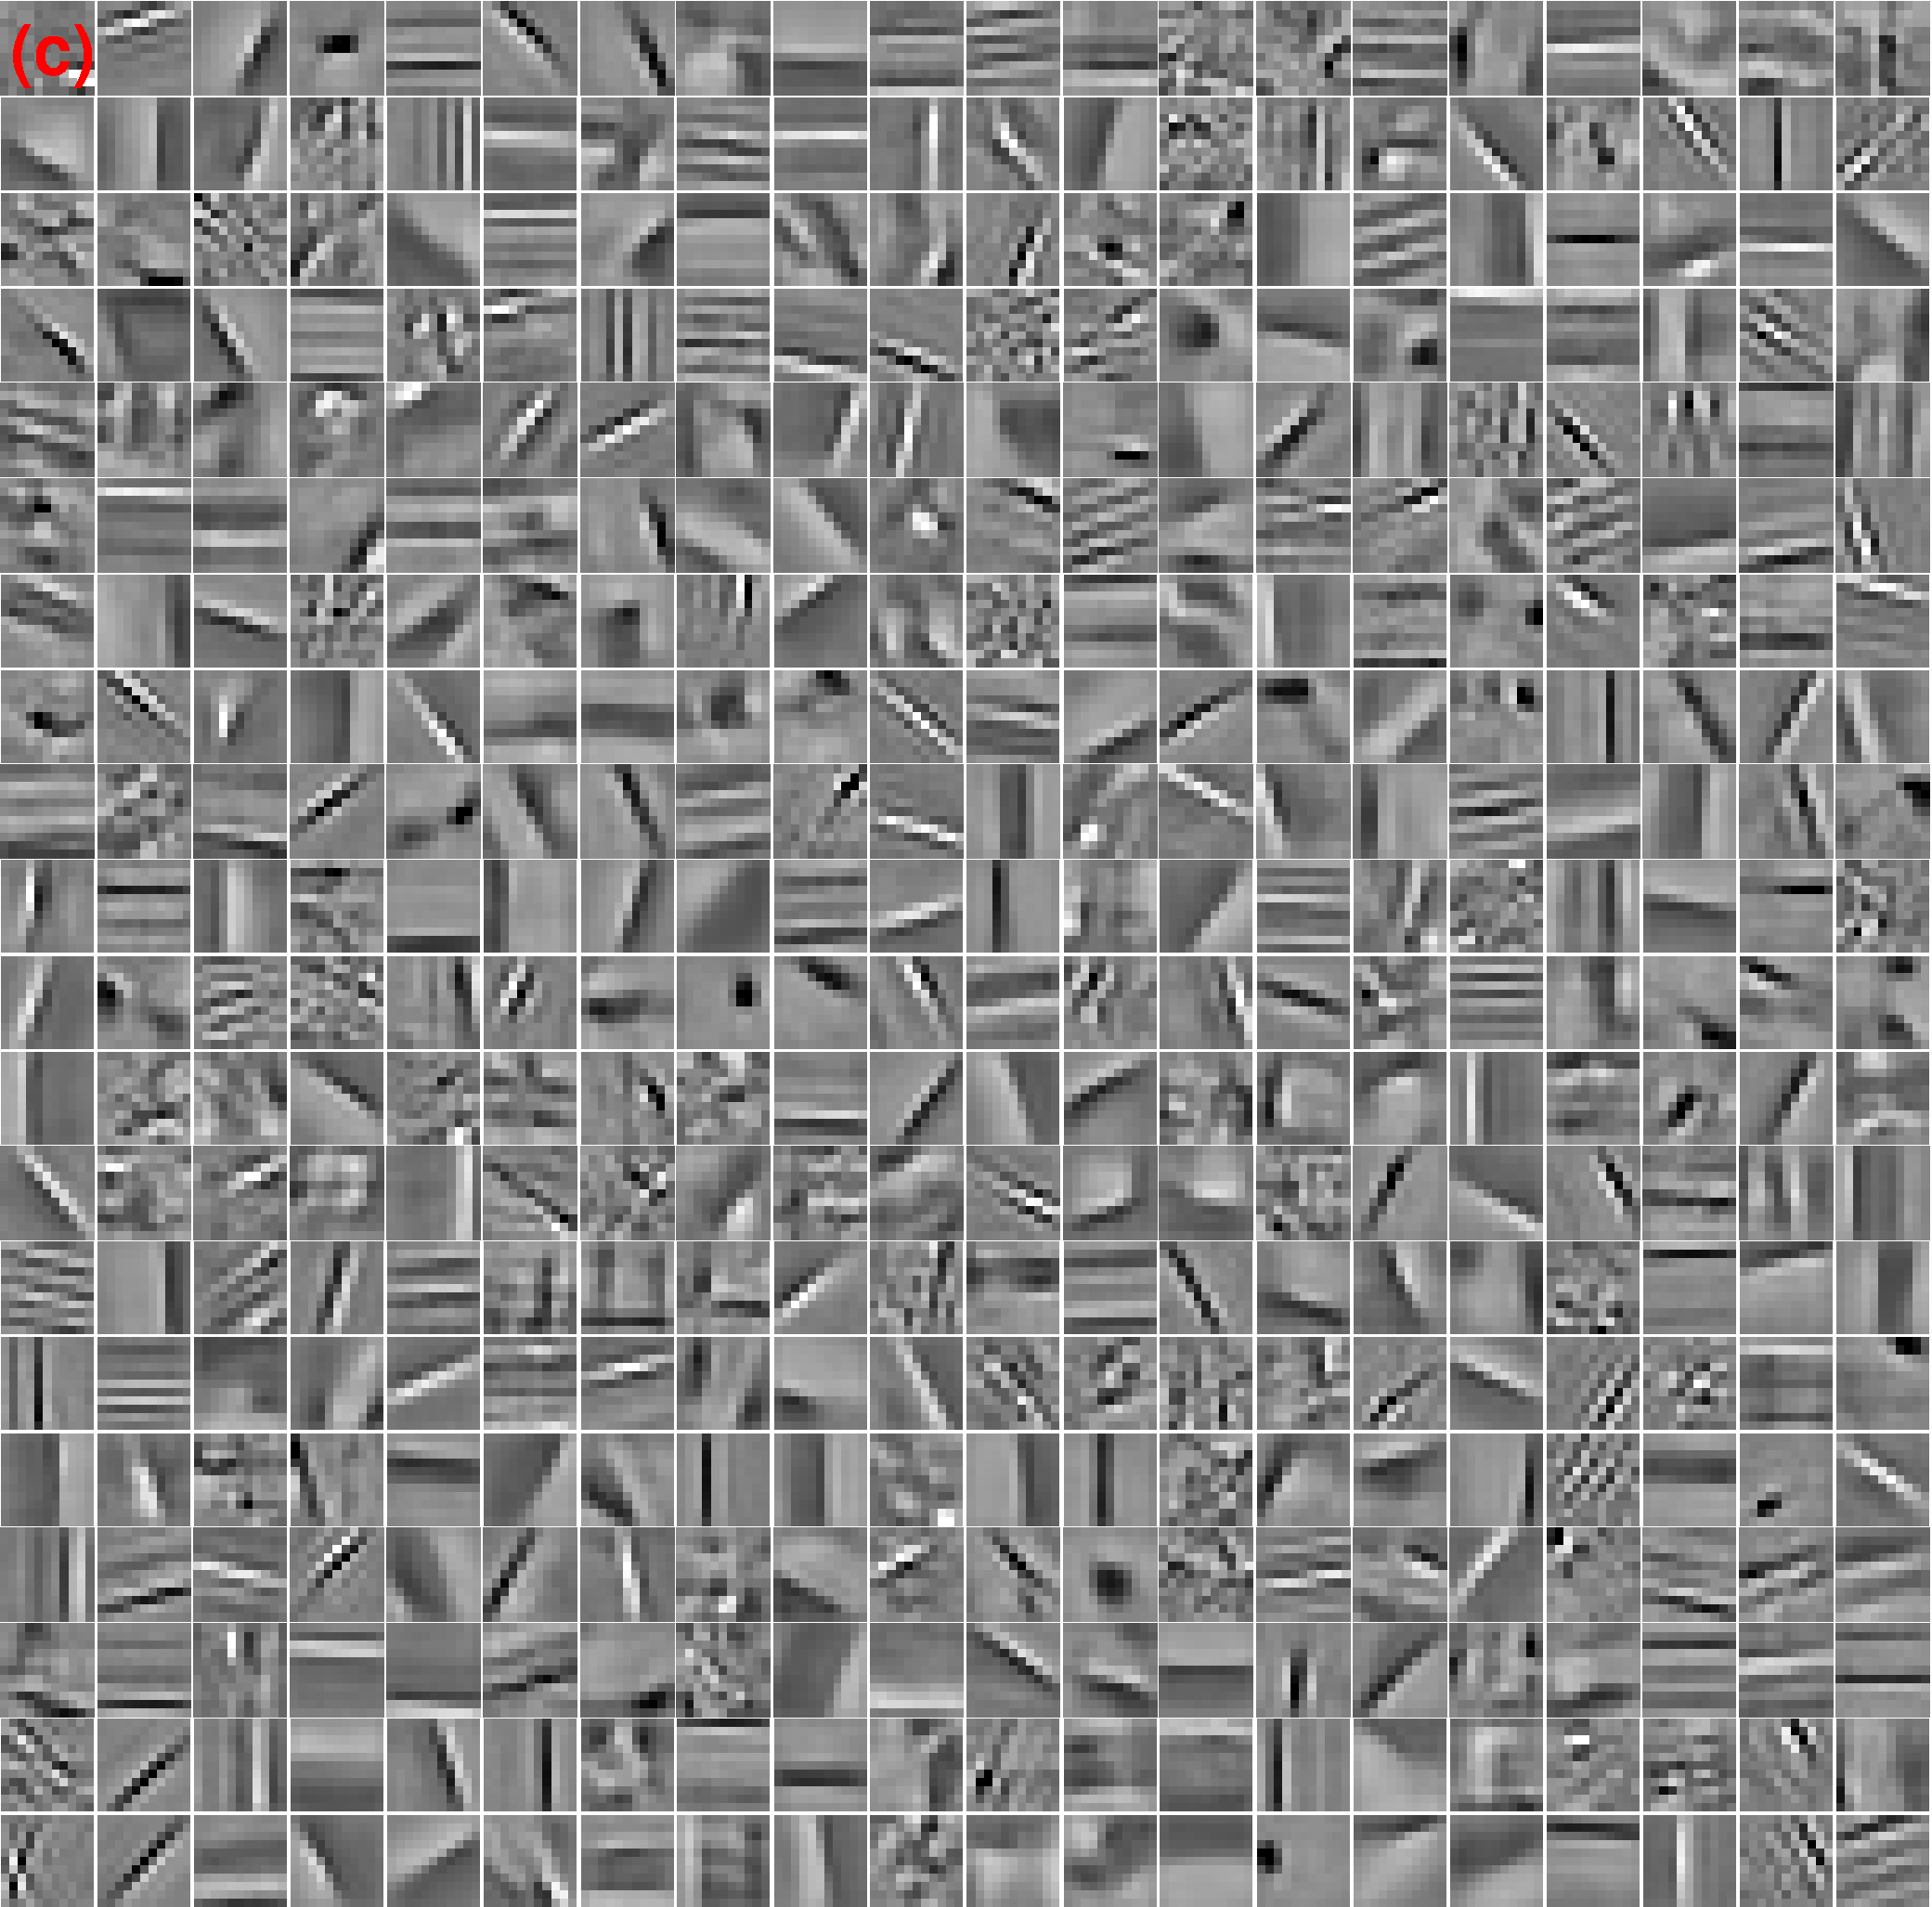
\includegraphics[width=1\linewidth]{figure/online400-filter.pdf}
\end{minipage}
    \\
    \\
    \\
    \resizebox{1\linewidth}{!}{
        \begin{tabular}{|c||c|c|c|c|c|c|c|c|c|c|}
            \cline{1-11}
            Image & 1 & 2 & 3 & 4 & 5 & 6 & 7 & 8 & 9 & 10 \\
            \hline
            PSNR by (a) & 29.58 & 28.19 & 29.44 & 29.63 & 28.89 & 29.33 & 28.13  & 30.14 & 27.42 & 30.89 \\
            \hline
            PSNR by (b) & 29.63 & 28.22 & 29.57 & 29.90 & 29.12 & 29.59 & 28.05  & 30.17 & 27.53 & 31.08 \\
            \hline
            PSNR by (c) & \textbf{30.24} & \textbf{28.34} & \textbf{29.95}  & \textbf{30.30} & \textbf{29.43} & \textbf{29.96} & \textbf{28.24} & \textbf{30.57} & \textbf{27.72} & \textbf{31.67} \\
            \hline
        \end{tabular} }

\caption{Filters learned from 1000 images by our method and the state of-the-art method~\cite{liu-2018-first}, and their corresponding reconstruction quality. (a) The under-complete dictionary ($11 \times 11 \times 100$) learned by~\cite{liu-2018-first}; (b) The under-complete dictionary ($11 \times 11 \times 100$) learned by the proposed method. (c) The over-complete dictionary ($11 \times 11 \times 400$) learned by the proposed method. These under-complete dictionaries, mainly composed of Gabor-like filters, can be seen as a subset of the represented over-complete dictionary, which also contains a number of low contrast image features.
\peter{Include these filters in the supplementary, but make them much bigger so that people can see the deltails.}
}
\label{fig:overCompleteDic}
\end{figure}

We demonstrate its capability on 1000 image patches with the size of $100 \times 100$, and learn $11 \times 11 \times 400$ over-complete dictionary, all of which are shown in Fig.~\ref{fig:overCompleteDic} . For a visual comparison, 100 learned filters by the same algorithm and its comparable approach are also represented for a visual comparison. As can be observed, both of the approaches learn visually similar under-complete dictionary, while the proposed method shows a $5 \times$ speedup over the competitive one. Furthermore, the learned over-complete dictionary is composed of the Gabor-like image features as represented in the under-complete dictionaries, as well as a number of low contrast features which are rarely existed in those under-complete dictionaries. These additional feature information would play an essential role to better represent the natural images, which can be demonstrated by the reconstruction quality shown in Fig.~\ref{fig:overCompleteDic}.

We further show a bottleneck revealed by the under-complete dictionary in the online-based CSC model. The left hand side of Fig.~\ref{fig:overComDicAndMinibatch} demonstrates that no more apparent progress could be observed when the number of training images is higher than a specific value for both of the online approaches. However, owing to more abundant filters, learning over-complete dictionary overcomes this bottleneck, and it shows a considerable improvement with regard to PSNR to have a sparse representation of the testing images during the learning process. This is also verified by applying these learned dictionaries to the image inpainting applications as discussed above.

\begin{figure}[h]
\centering
\begin{subfigure}{0.4\textwidth}
  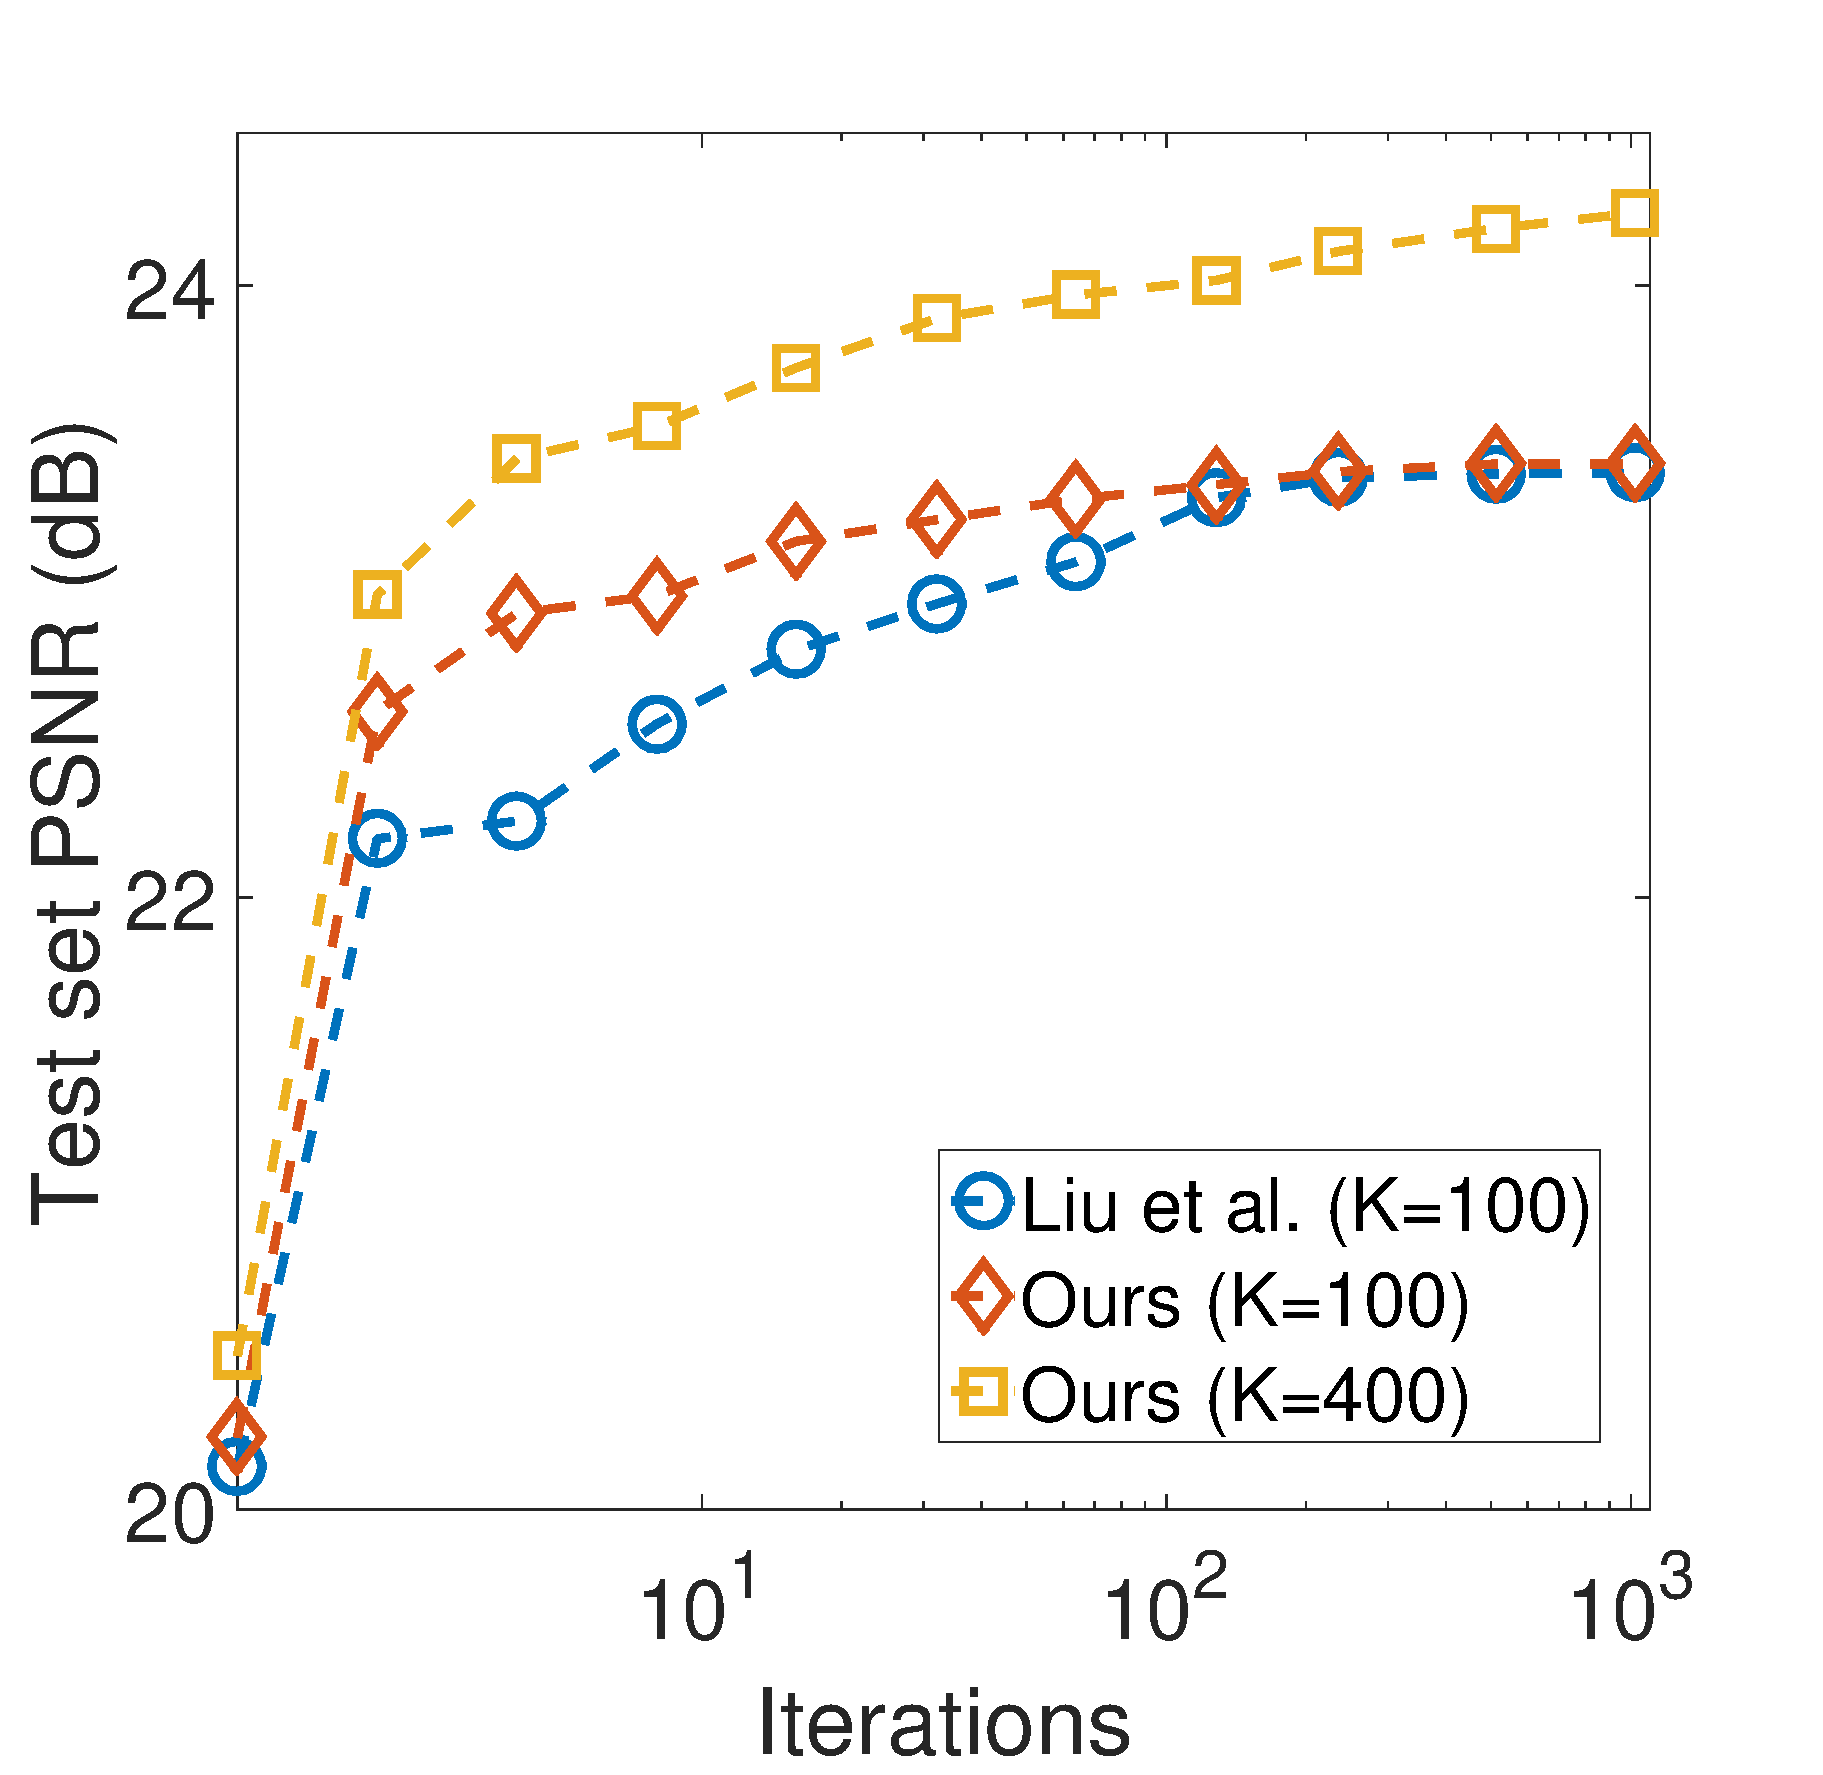
\includegraphics[width=1\linewidth]{figure/overComplete-ite.pdf}
\end{subfigure} 
\begin{subfigure}{0.55\textwidth}
  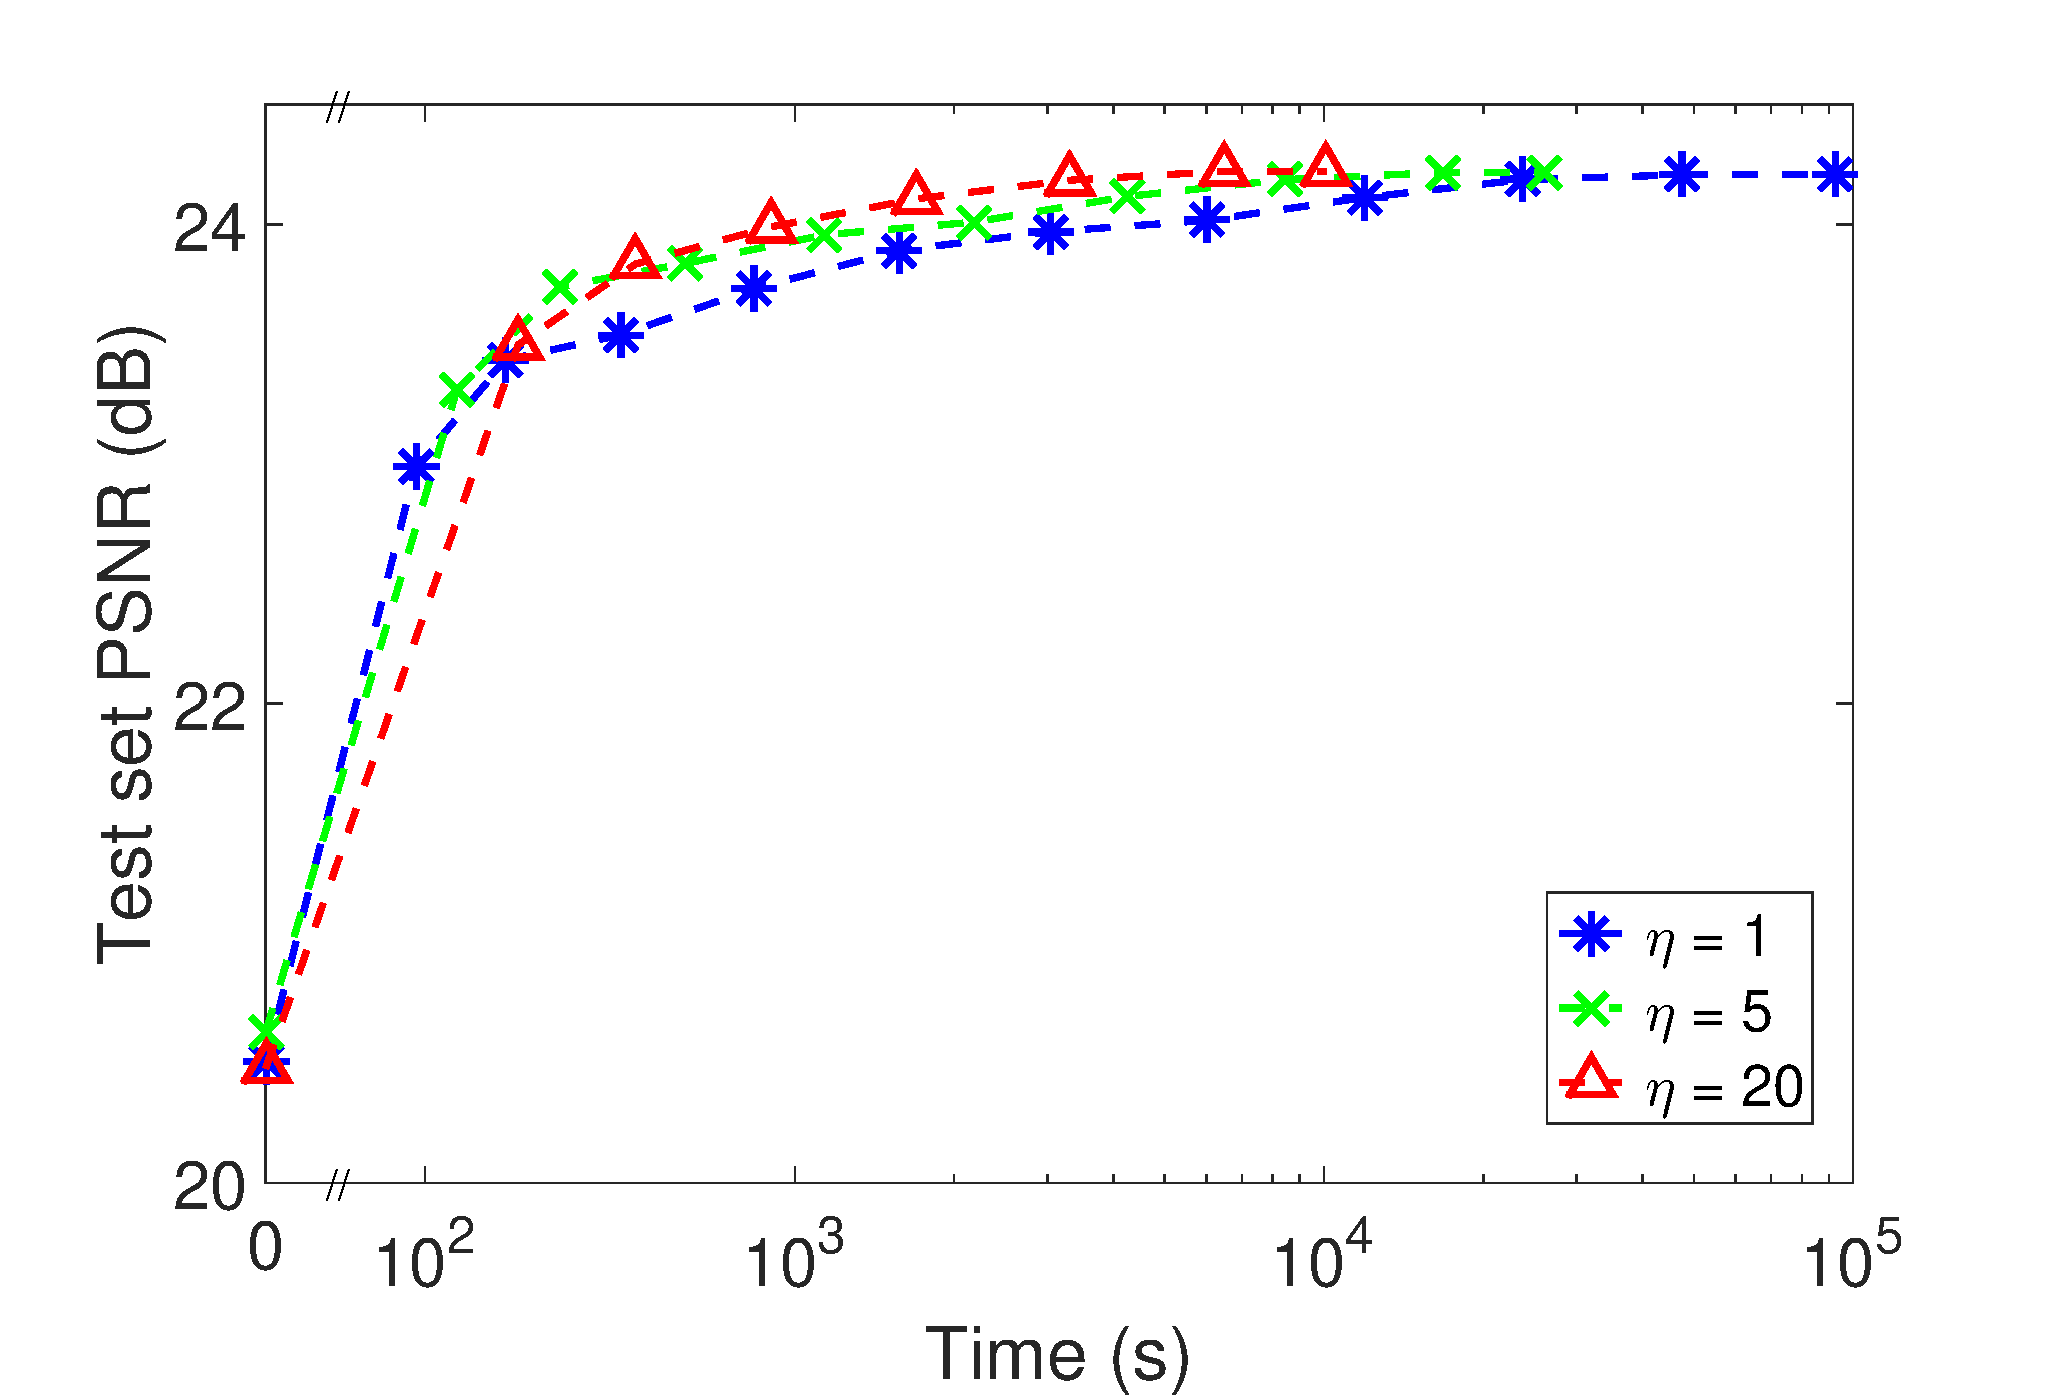
\includegraphics[width=1\linewidth]{figure/minibatch.pdf}
\end{subfigure}

\caption{Left: Testing PSNR for the compared method with $K=100$, and the proposed method with $K=100$ and $K=400$, respectively. Every iteration draws a single image from the training dataset. Right: Testing PSNR for the proposed method ($K=400$) with varying values of $\eta$.}
\label{fig:overComDicAndMinibatch}
\end{figure}

{\bfseries Mini-batching.} In practice, a mini-batching strategy would be preferred in order to gain advantage from modern parallel computing architectures. This is also a standard extension to stochastic optimization algorithms \cite{Takac2013, PCDM, SCSG}. We denote the mini-batch size as $\eta$. In the proposed algorithm, the time complexity for one step dictionary update will not increase linearly with the increase of $\eta$. Concretely speaking, updating $\code$ is implemented by Cholesky decomposition, and one computation of the matrix factorization can be applied to all of the currently selected batches. Herein, the complexity for doing updating $\code$ $\eta$ times all together is cheaper than $\eta$ times the complexity of updating one $\code$. In addition, the time complexity for updating $\filter$ is not affected by the value of $\eta$, which will be executed only once in each training step regardless of $\eta$. One exception is to update surrogate matrices, the complexity of which is $\eta$ linearly dependent, while this is not dominant in the runtime. The learned filters are examined on the test sets every $2^i$ iterations and the last iteration, where $i=0,1,...$. Note that larger $\eta$ will result in less number of iterations to process all 1000 images. The results for various mini-batch sizes are shown in Fig.~\ref{fig:overComDicAndMinibatch}. A larger mini-batch size shows a greater progress for first few training steps, though it takes additional running time and memory. Overall, mini-batched updates provides a more runtime efficient learning progress in online-based CSC model, and in the test examples, $\eta=20$ achieves one magnitude speedup over $\eta=1$ to reach a condition with the same level convergence.
